% !Mode:: "TeX:UTF-8"
%!TEX program  = xelatex

%\documentclass{cumcmthesis}
\documentclass[withoutpreface,bwprint]{cumcmthesis} %去掉封面与编号页

\usepackage{url}
\title{机场的出租车问题}
\tihao{C}
\baominghao{ 暂无 }
\schoolname{华中科技大学}
\membera{鲁镇仪}
\memberb{李欣航}
\memberc{蒋瀚锐}
\supervisor{暂无}
\yearinput{2020}
\monthinput{08}
\dayinput{19}

\begin{document}
\maketitle
\begin{abstract}
	现代社会中,人们在日常出行方式当中必然少不了出租车这个选项。如何让乘客和司机利益均得到保障是研究的问题。
	该文主要通过对宏观和微观两种情况建立数学模型,来得到有关出租车司机该如何进行决策的方法和机场管理部门应如何设置接车方式和对短途载客并再次返回的出租车给予“优先权”的具体解决方案。
	\par
	对于问题一,该文主要建立出宏观地图与司机等待模型,利用题目已知条件知道司机能看到的具体等待时间$t_{ \mathrm{wait}}$和计价方式还有出租车的平均收益$a$。用分段函数方式来求出了计价方式$f$的具体表达式。求出两种收益分别的表达式之后,直接比较这两个表达式,即可得到结果。
	\par
	对于问题二,选取郑州机场的目前的数据,有关于这部分数据均用爬虫取自于网上。利用过去半个小时之内离开飞机场和进入飞机场的车辆数,能够得到司机的平均等待时间$t_{ \mathrm{wait}}$的具体值,再利用郑州的出租车营业方案,得到计价方式$f$的具体表达式,这时候直接利用第一问的表达式即可完成此题。
	\par
	对于问题三,
	\par
	对于问题四,
	\par
	\keywords{元胞自动机 \quad 梯度下降}
\end{abstract}

\tableofcontents
\newpage
\section{问题重述}
\subsection{问题背景}
由于出租车的选择以及机场管理者所作出的决策对效率,时间,金钱均有着重大的影响。因此,对于机场管理者来说,对于加快机场外交通运营,增加司机收入,提高乘客舒适度,节约出行时间来说,提高机场出租车运营效率是具有重要意义的。
\begin{figure}[!h]
	\centering
	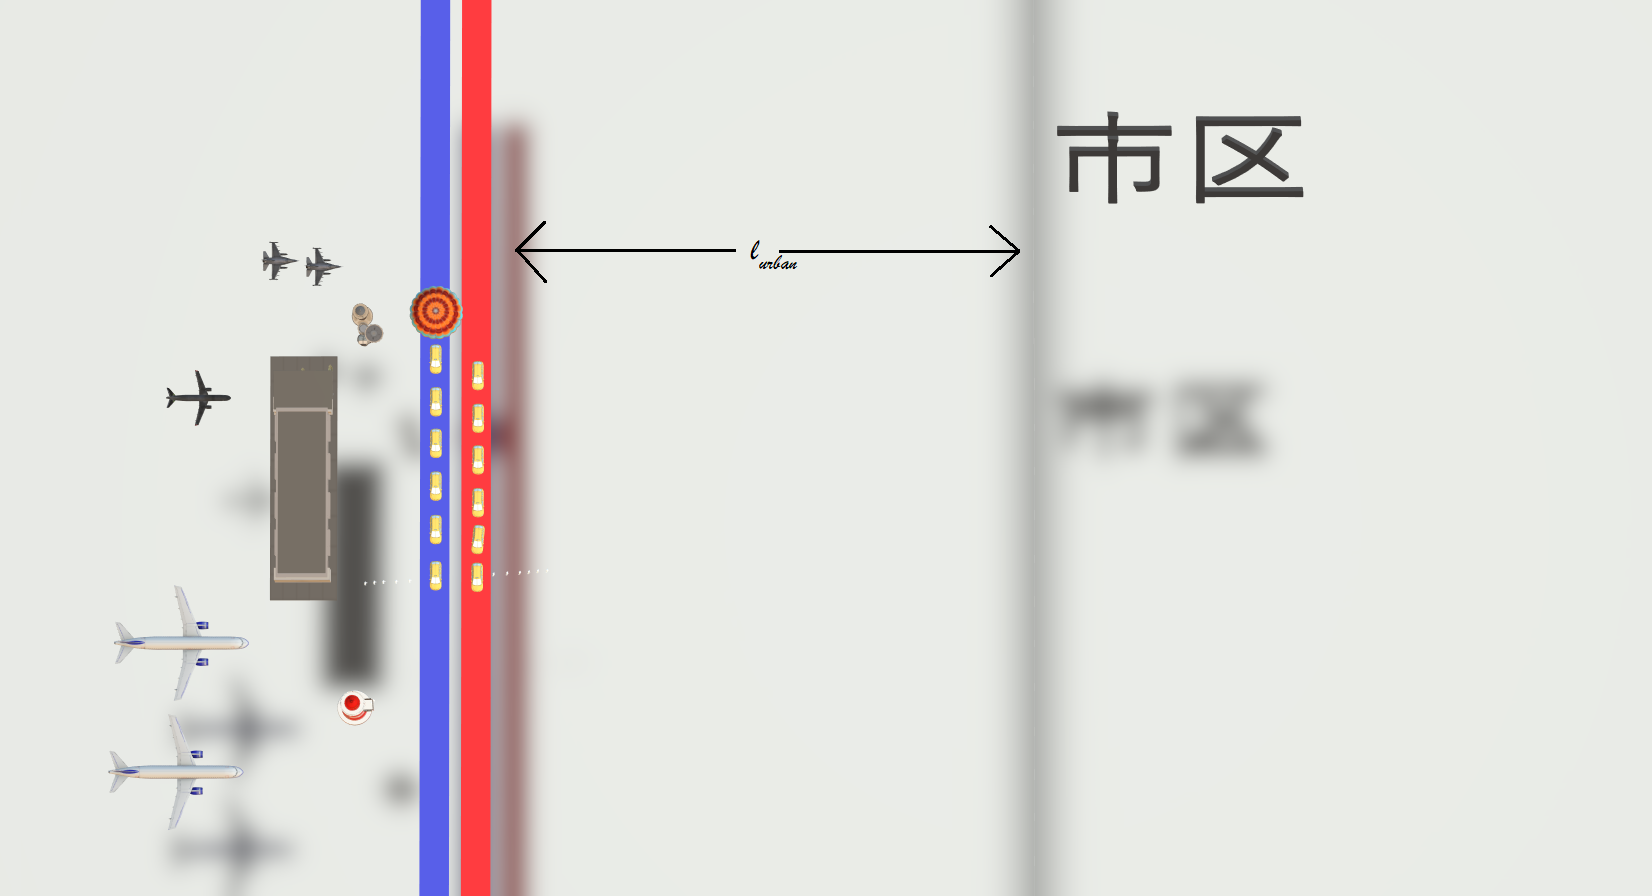
\includegraphics[width=0.8\textwidth]{Figure_1.png}
	\caption{市区,机场与排队等车模型示意图}
\end{figure}

\subsection{问题的提出}
该文章主要是研究不同情况下司机该如何来选择最优的方式和机场管理者该如何调整政策使得宏观效率最高。
由于出租车必须到指定的“蓄车池”排队等候,依“先来后到”排队进场载客,这导致司机有一个“排队时间成本”,如果不排队接客,则多出的时间就可以到市区接客。
但若直接去市区接客,则从机场到市区中间一段距离就是空置的。
\par
当然,为了解决这个问题,除了司机自身的判断之外,很重要的另外一点就是机场管理者的政策。
机场管理者设定不同的上下车点,司机接客的方式,对短途载客再次返回的出租车给予一定的“优先权”,均会影响到具体的效益以及收入情况。

\par
在问题一当中,题设较为简单,只需要建立出租车司机选择决策模型,并给出司机的选择策略即可,所以利用题目所给出的司机已知的条件。\par
也即大致的出租车司机排队等待时间加服务时间$t_{ \mathrm{wait}}$和出租车的计价方式$f$还有具体的城市到飞机场的距离$l_{\mathrm{urban}}$。\par
第一小问希望利用这些条件,能够得到最终司机分别在哪一种情况下选择哪一种方案的解析解。

\par
在问题二当中,题目直接要求对于一个具体城市的具体司机的具体选择,这需要考察网上的信息搜索能力,在第一问已经得到抽象的解析解的时候,题目要求只需要把具体数值代入表达式当中得到具有现实参考意义的解。

\par
在问题三当中,

\par
在问题四当中,

\newpage
\section{问题分析}
\subsection{问题一的分析}
问题一较为简单,因此只需要拟定各个不同的定义所代表的含义,目的在于给司机选定到底选择哪一个哪一种方案收益最高。虽然本问并没有给出具体数据,但仍然可以把一些量用字母替代。\par
考虑到司机是能够观察到具体还有多少乘客和出租车的,所以直接能够假定司机知道还需要等待多久的时间,这是合理的。由于出租车司机的收入司机也是知道的,所以可以假定市区出租车的平均收入。\par
通过这些条件,选择是否留在机场接客还是直接回市中心是通过比较两者的平均收益得到的。\par
这时候利用之前得到的出租车收益图函数即可得到最终目标的解析解。\par

\subsection{问题二的分析}
问题二需要寻找具体的城市具体分析,由于没有附录提供的任何数据,使用计算机技术在网上进行爬虫,记录并得到了郑州市的有关具体数据。\par
由于这些数据并不是能够直接得到第一问所设条件的具体值,因此得对这些数据进行处理以得到最终需要的值。\par
通过这些数据,代入第一问所得到的值,能够得到该机场出租车司机的具体选择方案。最终,通过数据依赖分析来分析模型的合理性和对相关因素的依赖性。\par

\subsection{问题三的分析}


\subsection{问题四的分析}



\newpage
\section{模型假设}
\begin{itemize}
	\item 认为城市内和城市外行车速度恒定。
	\item 认为在路上的时候没有堵车情况发生,不考虑出租车关于时间的计费。
	\item 前两问假设服务时间为定值。
	\item 假设一辆车只载送一位乘客。
	\item 假设空载费用损失为油费。
	\item 假设一个周期内出租车和乘客一一抵消。
	\item 假设使用92号汽油。
	\item 假设出租车使用汽油总是$1L$走$11.8$公里的距离。
\end{itemize}

\newpage
\section{符号系统}
\begin{center}
	\begin{tabular}{cc}
		\hline
		\makebox[0.3\textwidth][c]{符号} & \makebox[0.4\textwidth][c]{意义}                     \\ \hline
		$fee$                            & 出租车的计价收益                                     \\
		$t_{ \mathrm{wait}}$             & 出租车排队等待时间加服务时间                         \\
		$m_{\mathrm{start}}$             & 出租车起步价                                         \\
		$m_{\mathrm{oil}}$               & 每一公里出租车的油费价格                             \\
		$m_{\mathrm{night}}$             & 夜价提升价格量                                       \\
		$m_{\mathrm{aver}}$              & 在市区当中的平均收入                                 \\
		$l_{\mathrm{init}}$              & 出租车计价起步距离                                   \\
		$k$                              & 每公里计费价格                                       \\
		$l_{\mathrm{urban}}$             & 机场到高速路口的平均距离                             \\
		$l_{\mathrm{city}}$              & 高速路口到市中心的平均距离                           \\
		$v_{\mathrm{sub}}$               & 从机场到市区当中的郊区行车速度                       \\
		$v_{\mathrm{city}}$              & 出租车回到市区后平均速度                             \\
		$t_{\mathrm{city}}$              & 出租车回到市区后为完成机场订单仍需在城市中行车的时间 \\
		$t_{\mathrm{wait}}$              & 出租车排队等待时间与服务时间总和                     \\
		\hline
	\end{tabular}
\end{center}

注:未列出及重复符号以出现处为准

\newpage
\section{建模与求解}
\subsection{出租车的收益模型}
对于城市出租车,忽略其型号、车龄等差别,并假设每辆出租车参数相同。\par
在一个城市中,出租车管理中通常几种计费方式混合使用,不同情况下计费方式不同。在这里为简化模型,选取最常用的计费方式。该计费方式描述如下:\par
出租车起步价为$m_{\mathrm{start}}$元,在$l_{\mathrm{init}}$公里后开始按路程距离计价,每多一公里计费$k$元。夜价则在日价的起步价基础上增加$m_{\mathrm{night}}$元。\par
则白天时的出租车计价方式如下:\par
\begin{equation}
	fee(d,\mathrm{day})=\left\{
	\begin{array}{lr}
		m_{\mathrm{start}}                               & ,d<l_{\mathrm{init}}    \\
		m_{\mathrm{start}}+ k \cdot(l-l_{\mathrm{init}}) & ,d\ge l_{\mathrm{init}}
	\end{array}
	\right.
\end{equation}

夜晚时出租车计价方式如下:\par
\begin{equation}
	fee(d,\mathrm{night})=fee(d,\mathrm{day})+m_{\mathrm{night}}
\end{equation}

但在出租车行驶过程中,如果出现空载情况,司机需要承担一定损失。假设空载损失的主要部分是油费,且油费与行车距离成正比,系数为每公里出租车油费价格$m_{\mathrm{oil}}$:\par
\begin{equation}
	oilfee(d)=d\cdot m_{\mathrm{oil}}
\end{equation}

用matlab对白天情形下的$fee-d$函数关系与$oilfee-d$函数关系进行可视化,结果如下:\par
\begin{figure}[!h]
	\centering
	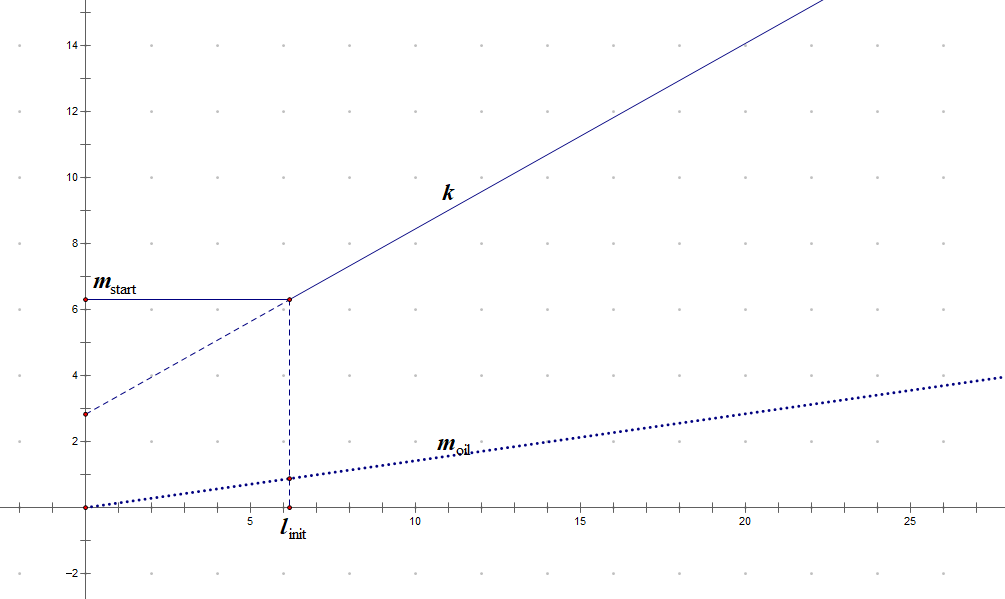
\includegraphics[width=0.8\textwidth]{Figure_2.png}
	\caption{出租车的收益函数图示}
\end{figure}

在前两问中,出租车总收益将由出租车计价收入$fee$与油费消耗$oilfee$构成,用符号简记为:
\begin{equation}
	sumfee(d)=fee(d)-oilfee(d)
\end{equation}

\subsection{问题一的建模与求解}
\subsubsection{模型准备}

只需要明确相同时间内排队载客后返回市区和空载返回市区这两种情况的平均收益该计算公式,司机便能够就是否排队问题做出决策。假定机场到市区的平均距离为$l_{\mathrm{urban}}$。从机场到市区行车速度为$v_{\mathrm{out}}$,市区中行车速度为$v_{\mathrm{city}}$。
\par

\subsubsection{模型的建立}

(1)首先明确要考虑的时间段。从选择排队载客后返回市区的方向对时间段进行刻画,整个时间段划分为三部分:

1.出租车排队等待时间与服务时间总和$t_{ \mathrm{wait}}$。

2.出租车从机场返回市区时间$t_{ \mathrm{return}}$,其计算方式为:
\begin{equation}
	t_{ \mathrm{return}}=\frac{l_{\mathrm{urban}}}{v_{\mathrm{sub}}}
\end{equation}

3.出租车回到市区后为完成机场订单仍需在城市中行车的时间$t_{\mathrm{city}}$。

记总时间为$t_{ \mathrm{sum}}$,其中:
\begin{equation}
	t_{ \mathrm{sum}}=t_{ \mathrm{wait}}+t_{ \mathrm{return}}+t_{\mathrm{city}}
\end{equation}

将该时间段对应到空载返回市区的情形,则有:

1.出租车从机场返回市区时间$t_{ \mathrm{return}}$。

2.出租车返回市区后接客时间$t_{ \mathrm{wait}}+t_{\mathrm{city}}$

下面将根据上述上述时间划分对两种选择的平均收益进行计算。

(2)若司机选择排队载客后返回市区,那么总时间段内平均收益的计算方法如下:\par
\begin{equation}
	aveincome1=\frac{sumfee(l_{\mathrm{urban}}+v_{\mathrm{city}} \cdot t_{\mathrm{city}})}{t_{ \mathrm{sum}}}
\end{equation}
\par
上式中假定等待时间与服务时间无收入与损失,分子中总收入为机场中接到的一单收入。

\par \par
(3)若司机选择空载返回市区,那么总时间段内平均收益的计算方法如下:\par
\begin{equation}
	aveincome2=\frac{m_{\mathrm{aver}}\cdot(t_{\mathrm{wait}}+t_{\mathrm{city}})-oilfee(l_{\mathrm{urban}})}{t_{ \mathrm{sum}}}
\end{equation}

上式中$m_{\mathrm{aver}}$表示出租车司机在城市内每小时平均收入(考虑了油费损失)。分子中总收入为市区中行车收入减去从机场返回市区的油费消耗。\par
\par

我们只需比较这两个的大小:

1.若$aveincome1>aveincome2$,应选择排队载客后返回市区。

2.若$aveincome1<aveincome2$,应选择空载返回市区。

下面解该不等式:\par
\begin{equation}
	\left\{
	\begin{array}{l}
		aveincome1>aveincome2                                                                                                       \\
		aveincome1=\frac{sumfee(l_{\mathrm{urban}}+v_{\mathrm{city}} \cdot t_{\mathrm{city}})}{t_{ \mathrm{sum}}}                   \\
		aveincome2=\frac{m_{\mathrm{aver}}\cdot(t_{\mathrm{wait}}+t_{\mathrm{city}})-oilfee(l_{\mathrm{urban}})}{t_{ \mathrm{sum}}} \\
		sumfee(l)=fee(l)-oilfee(l)                                                                                                  \\
		oilfee(l)=l\cdot m_{\mathrm{oil}}
	\end{array} \right.
\end{equation}

解得:
\begin{equation}
	t_{\mathrm{wait}}< \frac{fee(l_{\mathrm{urban}}+v_{\mathrm{city}} \cdot t_{\mathrm{city}})-m_{\mathrm{oil}}\cdot v_{\mathrm{city}} \cdot t_{\mathrm{city}}}{m_{\mathrm{aver}}} -t_{\mathrm{city}}
\end{equation}
我们记这个特殊的时间点为判断等待时间$t_0$:
\begin{equation}
	t_0=  \frac{fee(l_{\mathrm{urban}}+v_{\mathrm{city}} \cdot t_{\mathrm{city}})-m_{\mathrm{oil}}\cdot v_{\mathrm{city}} \cdot t_{\mathrm{city}}}{m_{\mathrm{aver}}} -t_{\mathrm{city}}
\end{equation}\par
等待时间$t_{\mathrm{wait}}$比判断等待时间$t_0$小时,选择排队载客后返回市区;当等待时间$t_{\mathrm{wait}}$比判断等待时间$t_0$大时,司机空载返回市区更加划算。\par

那么问题转化为如何计算等待时间与服务时间总和$t_{\mathrm{wait}}$。由题意可知司机可获取的信息为航班信息与蓄车池中出租车数量。该模型将通过这两个变量计算出等待时间与服务时间总和$t_{\mathrm{wait}}$。

为建立该计算模型,先定义三个速度:

1.蓄车池进车速度$v_{\mathrm{in}}$,表示每分钟进入蓄车池的车辆数。假设其于白天为一定值,于晚上为另一定值。

2.服务速度$v_{\mathrm{out}}$,表示每分钟离开蓄车池的车辆数。假设其于单队列单服务口情形下为定值。

3.乘客队列增长速度$v_{\mathrm{pin}}$,表示每分钟乘客队列增长人数。假设每时刻(航班到达时刻间隔为30分钟)到达的航班数量为$n_{\mathrm{fly}}$,每辆航班上乘客为300人,乘客选择乘坐出租车的比例为$\alpha$。那么通过下式对乘客队列增长速度进行计算:
\begin{equation}
	v_{\mathrm{pin}}=\frac{n_{\mathrm{fly}}\cdot 300 \cdot \alpha}{30}
\end{equation}

对于3个速度大小,会有13种情况。下图用图示法进行划分,其中样本点到3个关键点的距离用来表示其3个速度大小。

%这里插入一张图片
\begin{figure}[!h]
	\centering
	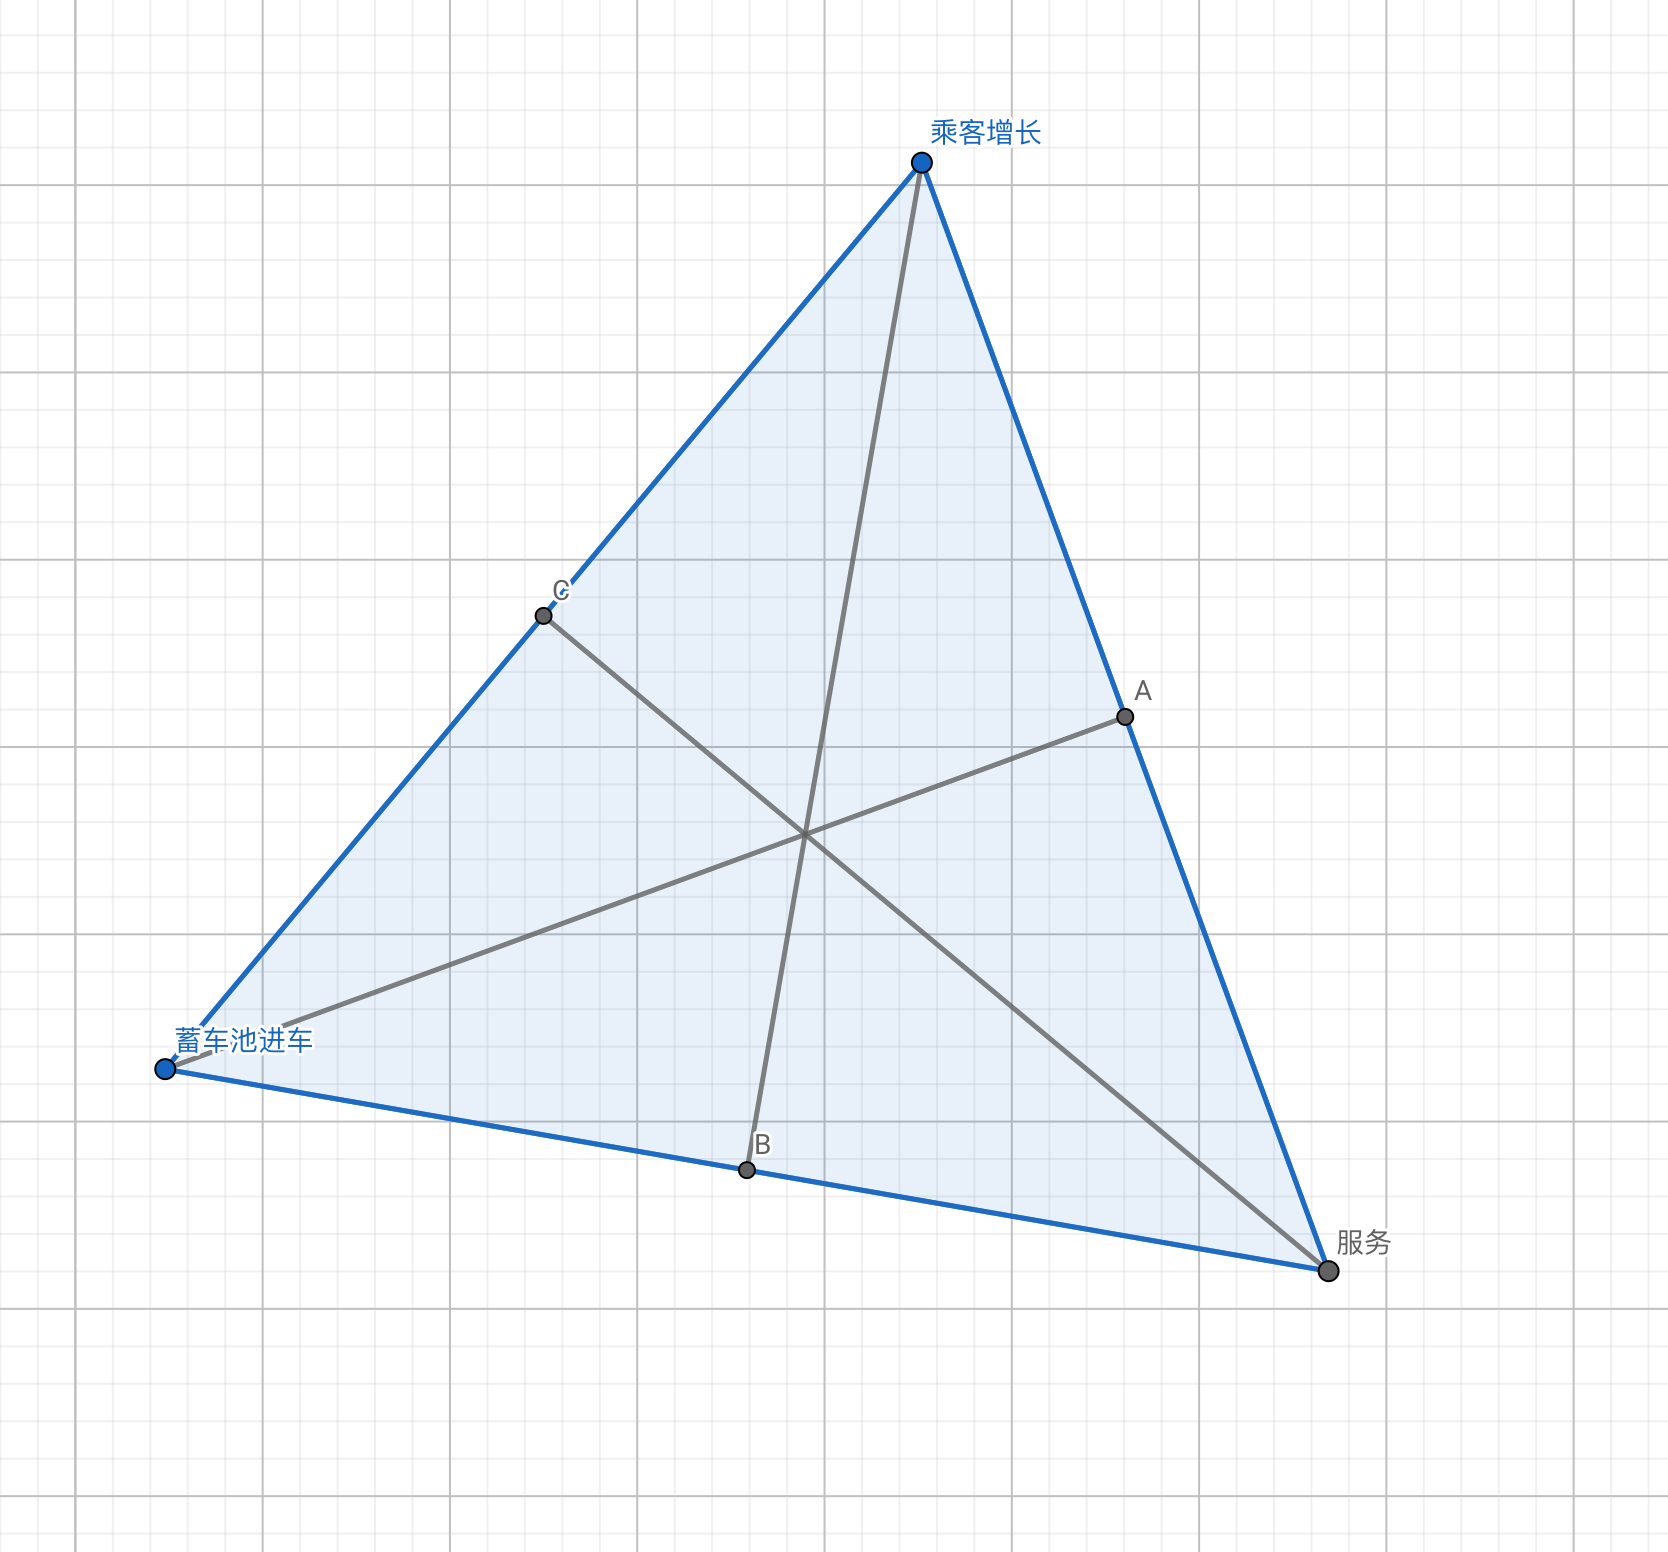
\includegraphics[width=0.8\textwidth]{等待时间计算模型.jpg}
	\caption{出租车的收益函数图示}
\end{figure}

13种情况分别为6块区域,6根分界线,1个中心点。对各个情况单独讨论,可发现会出现下述两种现象:

1.人堆积,随时间增长,乘客队列不断增长。

2.车堆积,随时间增长,蓄车池里车辆数量不断增长。

下列表格详细描述了各个情况:

\begin{center}
	\begin{tabular}{cc}
		\hline
		\makebox[0.3\textwidth][c]{情形}                    & \makebox[0.4\textwidth][c]{结果} \\ \hline
		$v_{\mathrm{pin}}>v_{\mathrm{in}}>v_{\mathrm{out}}$ & 人堆积,车堆积                   \\
		$v_{\mathrm{pin}}>v_{\mathrm{out}}>v_{\mathrm{in}}$ &
		人堆积                                                                                 \\
		$v_{\mathrm{pin}}>v_{\mathrm{in}}=v_{\mathrm{out}}$ & 人堆积                           \\
		$v_{\mathrm{pin}}=v_{\mathrm{in}}>v_{\mathrm{out}}$ & 人堆积,车堆积                   \\
		$v_{\mathrm{pin}}=v_{\mathrm{out}}>v_{\mathrm{in}}$ & 人堆积                           \\
		$v_{\mathrm{pin}}=v_{\mathrm{out}}=v_{\mathrm{in}}$ & 不堆积                           \\
		$v_{\mathrm{in}}>v_{\mathrm{pin}}>v_{\mathrm{out}}$ & 人堆积,车堆积                   \\
		$v_{\mathrm{in}}>v_{\mathrm{out}}>v_{\mathrm{pin}}$ & 车堆积                           \\

		$v_{\mathrm{in}}>v_{\mathrm{pin}}=v_{\mathrm{out}}$ &
		车堆积                                                                                 \\
		$v_{\mathrm{in}}=v_{\mathrm{out}}>v_{\mathrm{pin}}$ &
		车堆积                                                                                 \\

		$v_{\mathrm{out}}>v_{\mathrm{pin}}>v_{\mathrm{in}}$ &
		人堆积                                                                                 \\
		$v_{\mathrm{out}}>v_{\mathrm{in}}>v_{\mathrm{pin}}$ &
		车堆积                                                                                 \\
		$v_{\mathrm{out}}>v_{\mathrm{pin}}=v_{\mathrm{in}}$ &
		不堆积                                                                                 \\

		\hline
	\end{tabular}
\end{center}

用上图表示结果为:
%此处插入图片
\begin{figure}[!h]
	\centering
	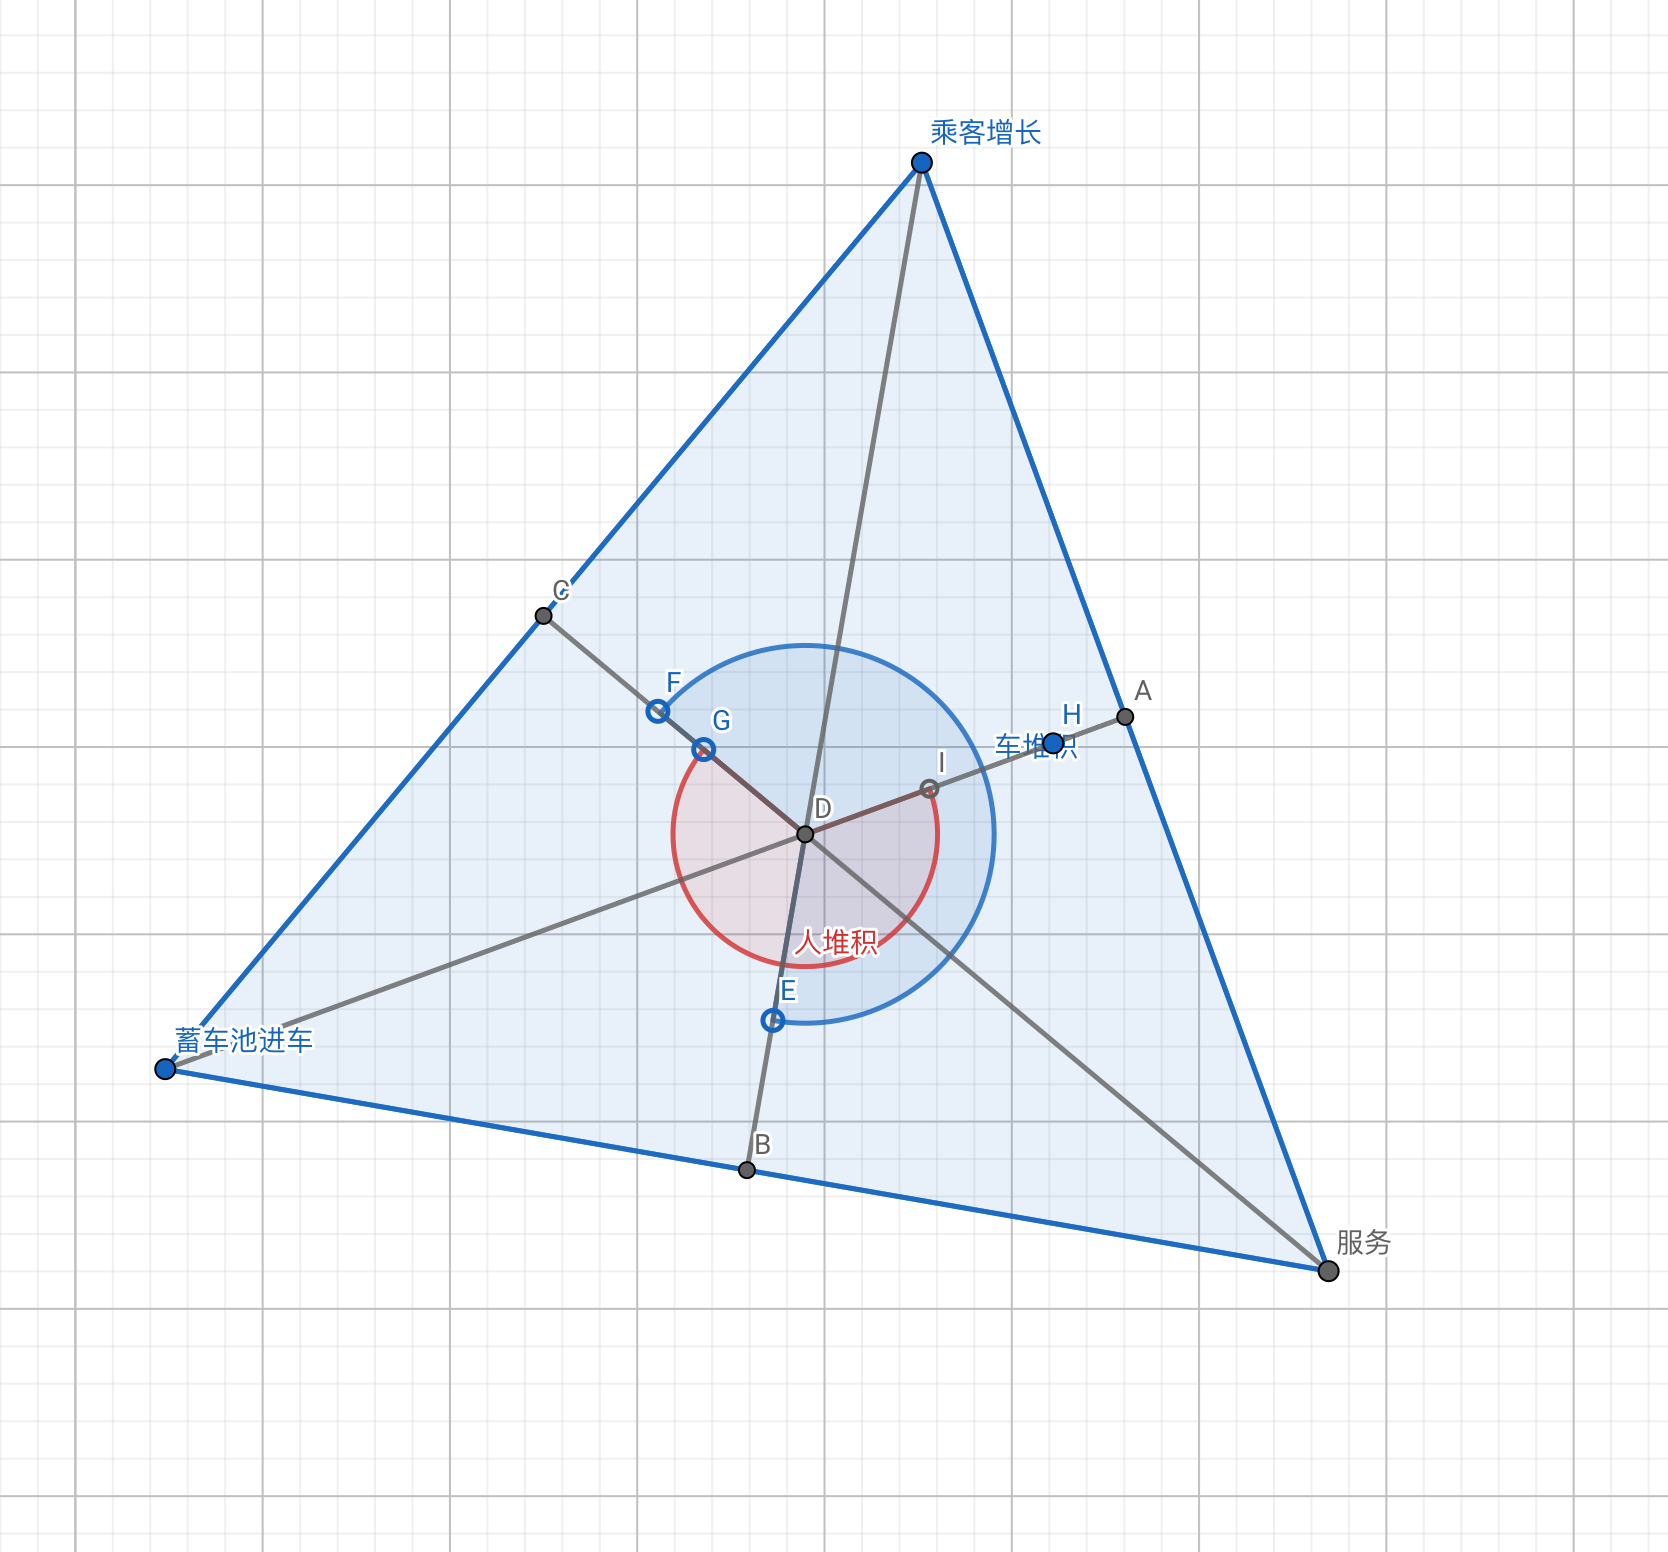
\includegraphics[width=0.8\textwidth]{等待时间计算模型2.jpg}
	\caption{出租车的收益函数图示}
\end{figure}
\newpage
将各个情形分别讨论之后,便能够着手进行等待时间加服务时间总和$t_{\mathrm{wait}}$的计算:

1.不堆积或人堆积时:
\begin{equation}
	t_{\mathrm{wait}}=\frac{n}{v_{\mathrm{out}}}
\end{equation}
其中$n$为蓄车池中出租车数量。

2.人不堆积而车堆积时:
\begin{equation}
	t_{\mathrm{wait}}=\frac{n}{v_{\mathrm{pin}}}
\end{equation}

\newpage
\subsection{问题二的建模与求解}
\subsubsection{模型的建立}

在郑州机场出租车秩序管理站上可以查询到实时的数据。\par
每个时刻蓄车池里面均有许多车辆在里面。利用数据,可以得到如下的统计图:\par
\begin{figure}[!h]
	\centering
	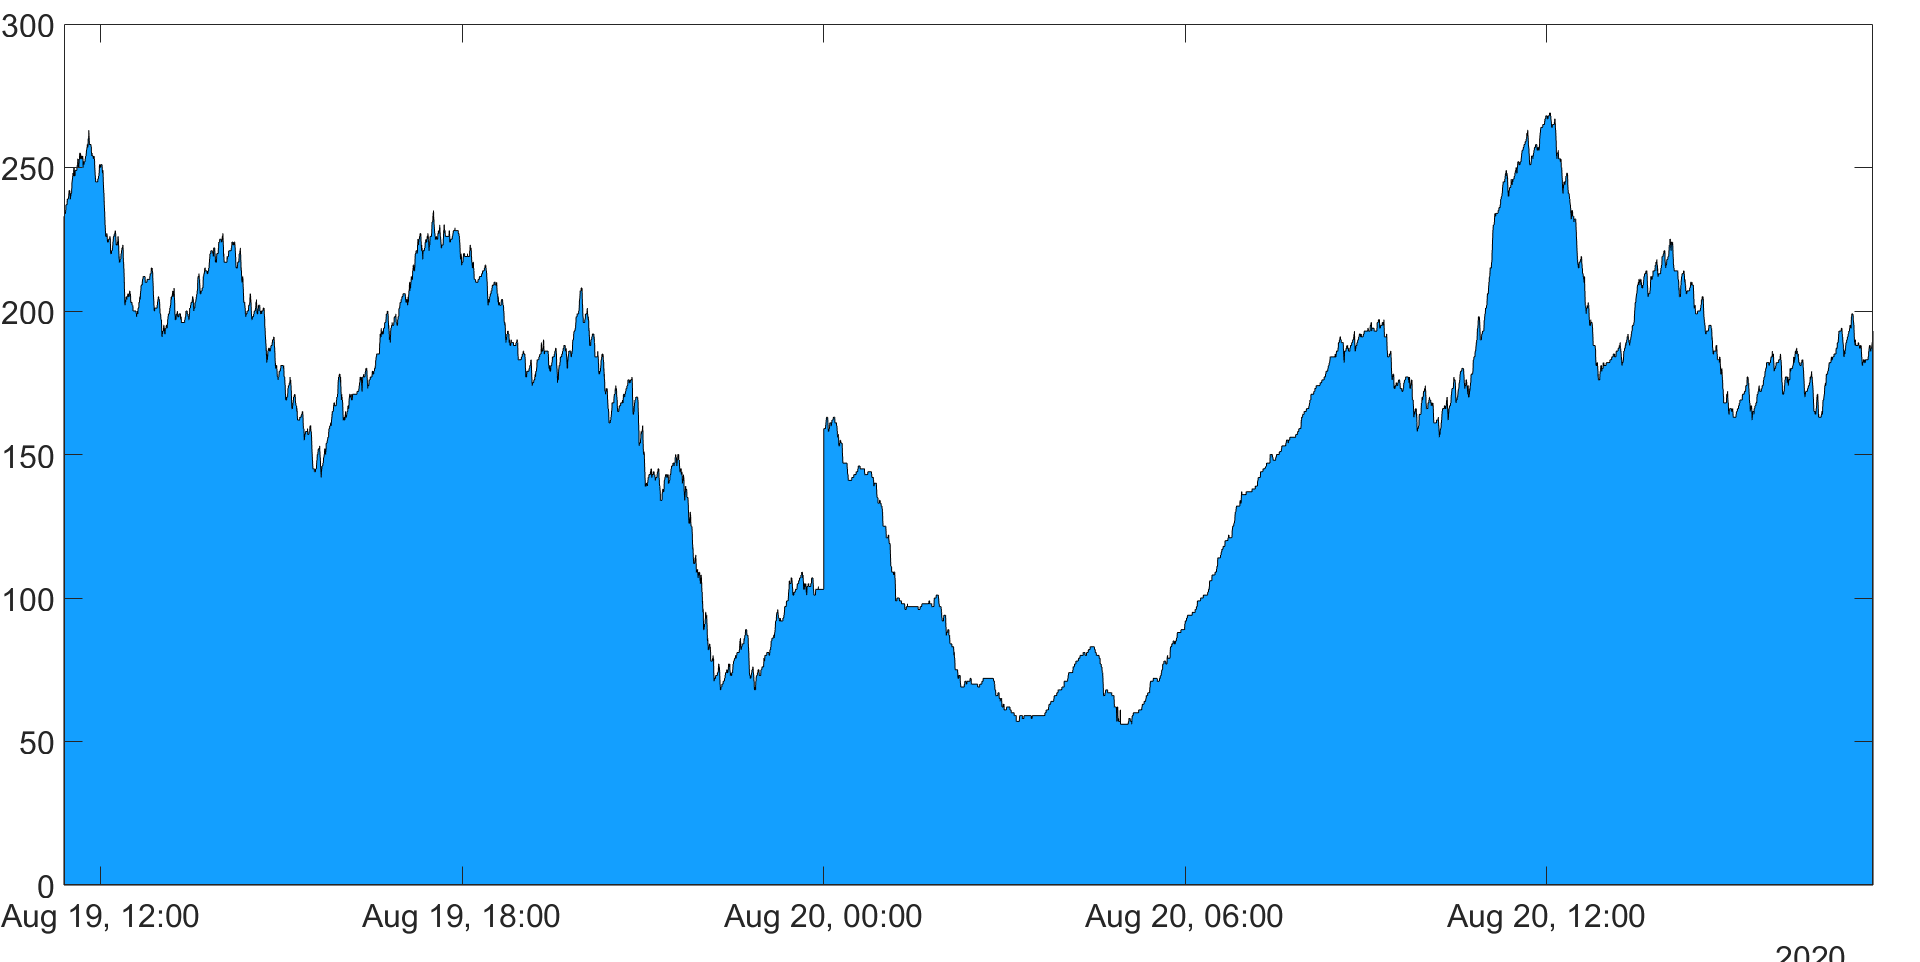
\includegraphics[width=0.9\textwidth]{Figure_3.png}
	\caption{场内待运车辆数统计图}
\end{figure}
还可以得到每一个时刻汽车出站运载的个数:\par
\begin{figure}[!h]
	\centering
	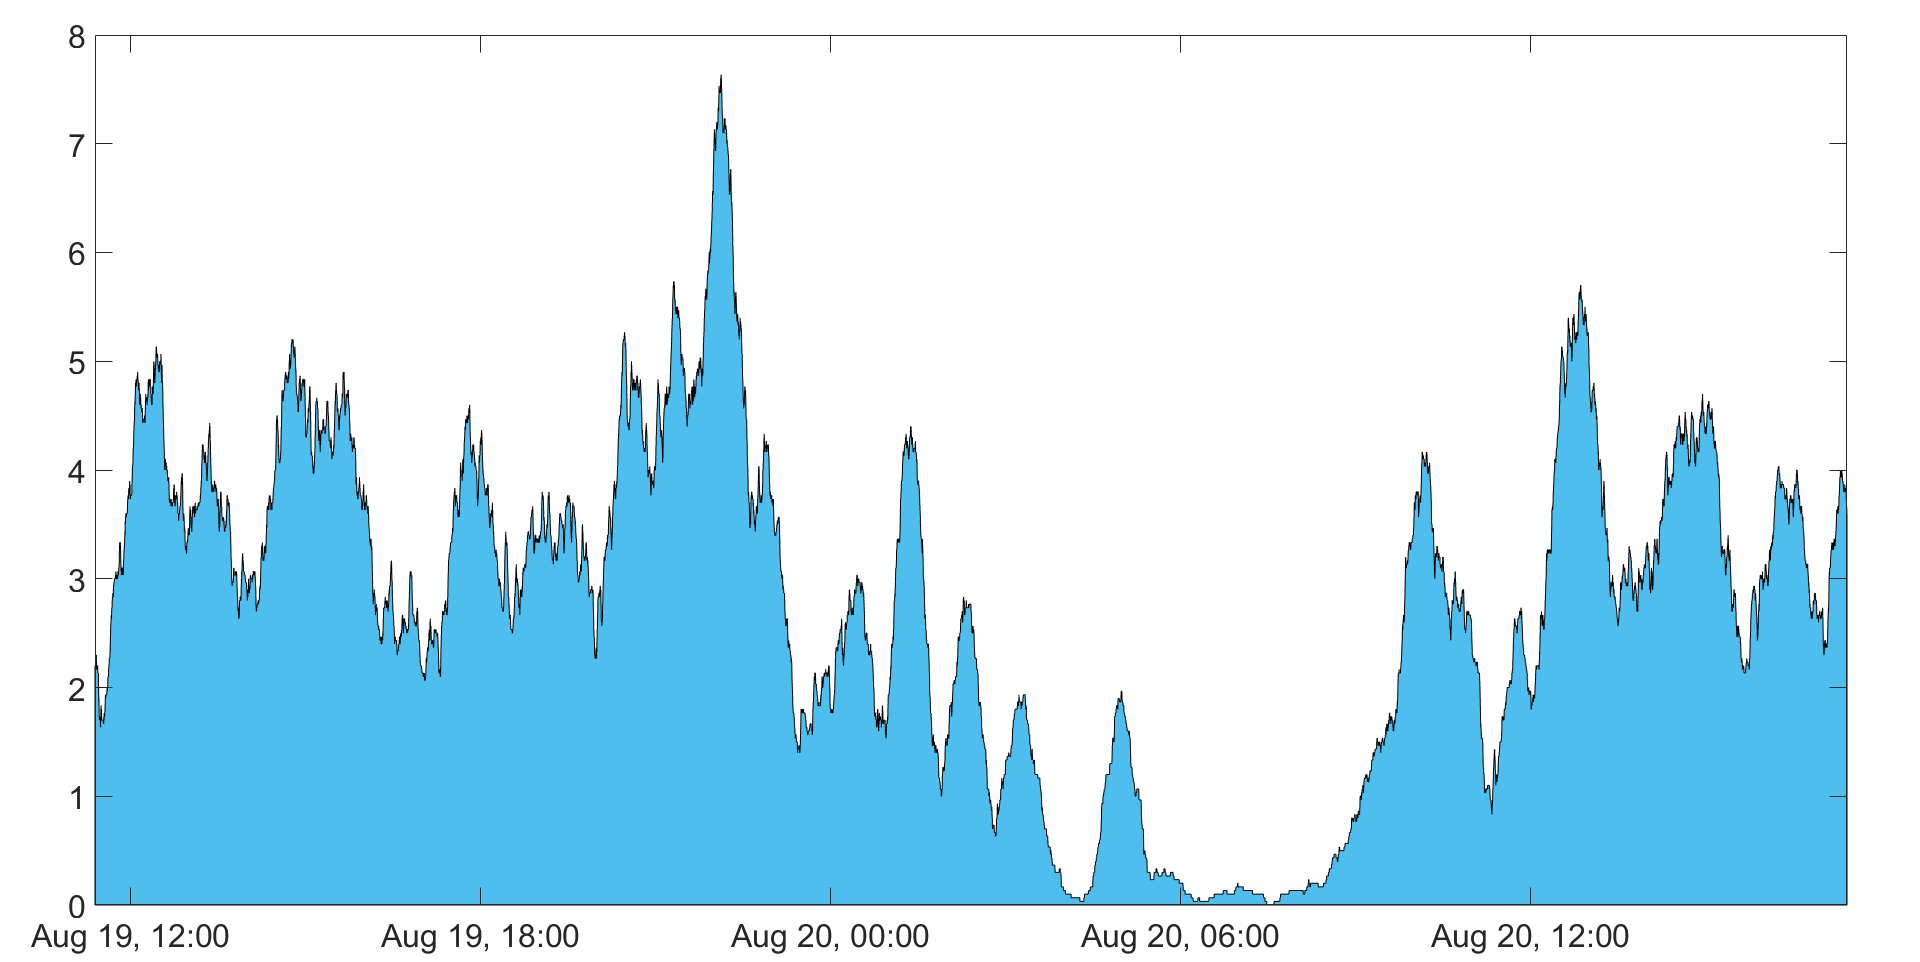
\includegraphics[width=0.9\textwidth]{Figure_4.png}
	\caption{运客速度统计图(单位:辆/min)}
\end{figure}

将场内待运车辆数写成关于时间$t$(单位:min)的表达式:$\eta(t)$。\par
再将出站车辆数写成关于时间$t$(单位:min)的表达式:$\theta(t)$\par
要求出$t_{\mathrm{wait}}$的大小,只需要一个积分方程。假设这个时候的时间点为$t$,则上面函数以及$t_{\mathrm{wait}}$满足约束式:\par
\begin{equation}
	\eta(t)=\int_{t}^{t+t_{\mathrm{wait}}}\theta(t)\mathrm dt
\end{equation}
由于$\theta(t)$无具体解析表达式,是统计得到的图表。有式子变换:\par
\begin{equation}
	\eta(t)=\int_{t}^{t+t_{\mathrm{wait}}}\theta(t)\mathrm dt\approx \sum_{i=0}^{[t_{\mathrm{wait}}]}{\theta(t+i)}
\end{equation}
找到满足条件的$t_{\mathrm{wait}}$,使得成立约束式:\par
\begin{equation}
	\sum_{i=0}^{t_{\mathrm{wait}}}{\theta(t+i)}\leq\eta(t) \leq\sum_{i=0}^{t_{\mathrm{wait}}+1}{\theta(t+i)}\quad\quad ( t_{\mathrm{wait}}\in \mathbb{N}^*)
\end{equation}\par
解出来的结果用面积统计图表示出来为:\par
\begin{figure}[!h]
	\centering
	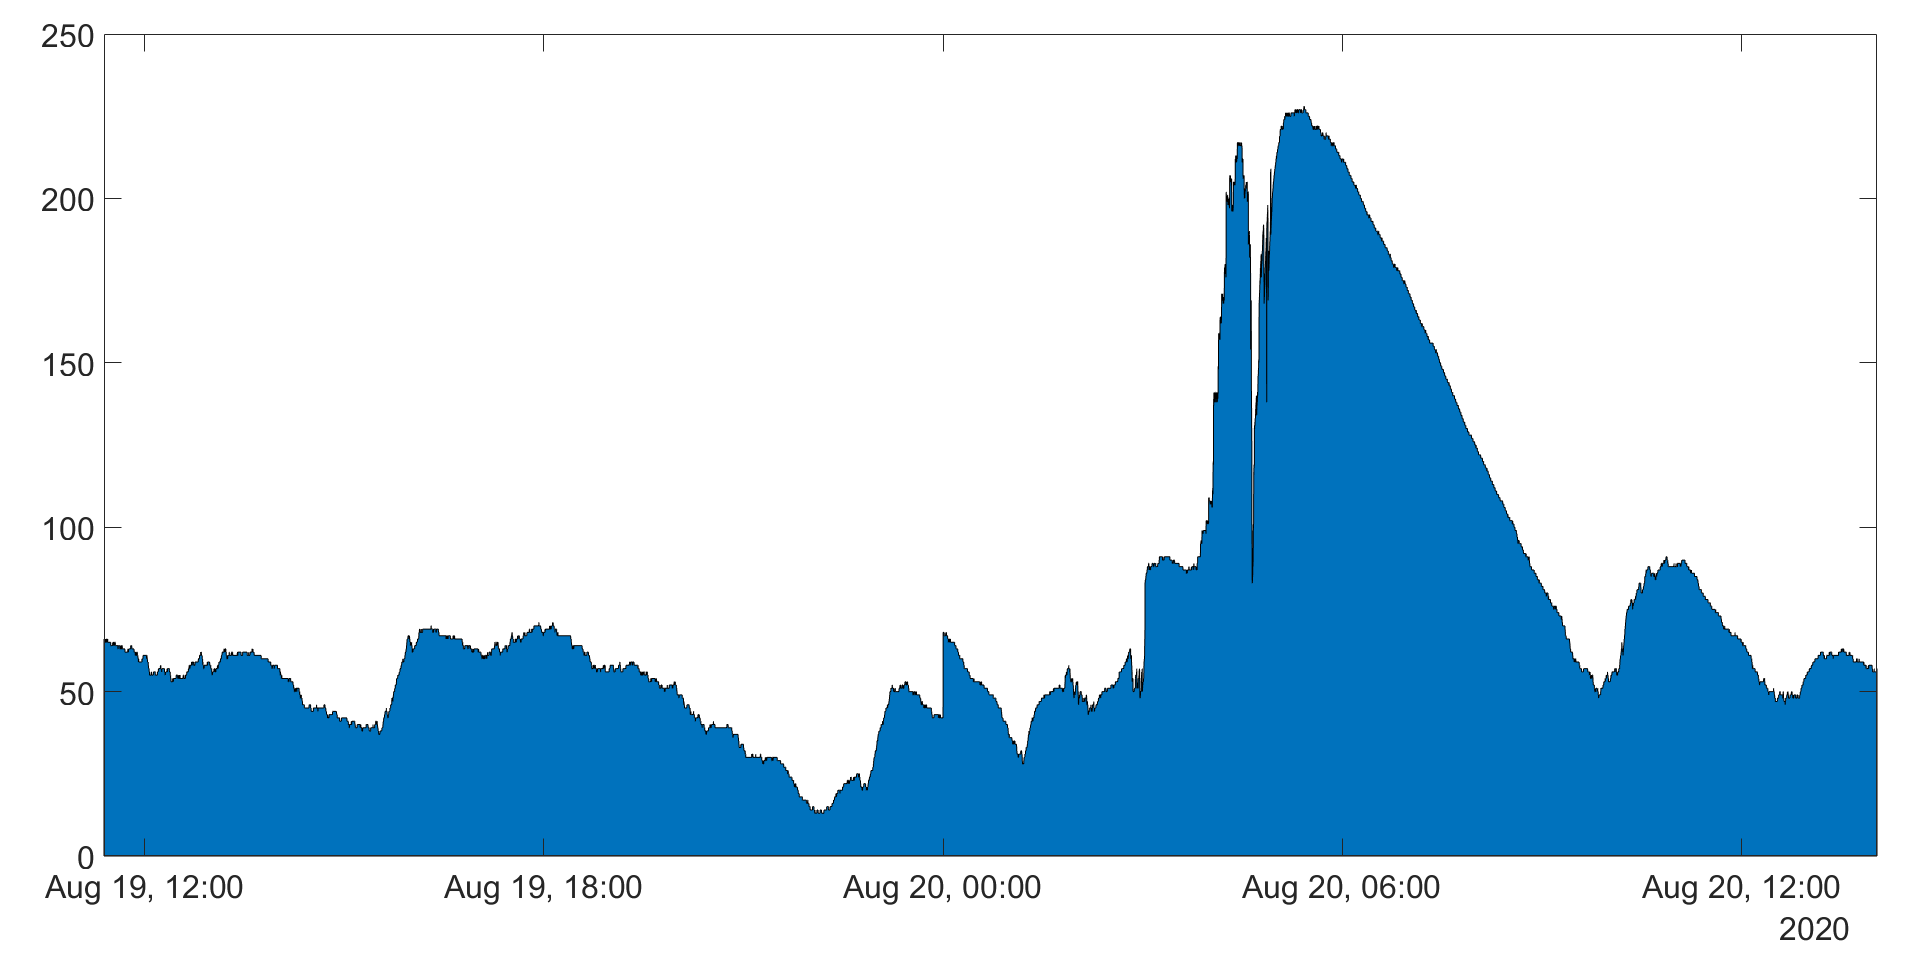
\includegraphics[width=1\textwidth]{Figure_5.png}
	\caption{等待时间统计图(单位:min)}
\end{figure}

\subsubsection{模型的求解}

目前再网络上能够找寻到的数据有:郑州司机的日均收入:$400$元人民币。按照每天工作$8$个小时计算,即每分钟$\frac{5}{6}$元人民币。也即$m_{\mathrm{aver} }= \frac{5}{6}$元。\par

这时候,查询郑州的出租车价格信息网得知,价格费用与路程的关系为:\par
\begin{equation}
	\mathrm{fee}(l)=\left\{
	\begin{array}{ll}
		c_0,                           & d \leq 2km \\
		c_0+1.5\cdot \left(l-2\right), & 2< d       \\
	\end{array}
	\right.
\end{equation}
$c_0$在白天$8$元,在晚上$10$元。\par
而这时候,查询郑州的汽油价格信息网得知,92号汽油每一升为$5.60$元,那么,每公里价格为$0.4746$元\par
查询高速路行车速度得知:平均速度为$100\mathrm{km/h}$即$\frac{5}{3}\mathrm{km/min} $\par
查询市区行车速度得知:平均速度为$30\mathrm{km/h}$即$0.5\mathrm{km/min} $\par
\begin{figure}[!h]
	\centering
	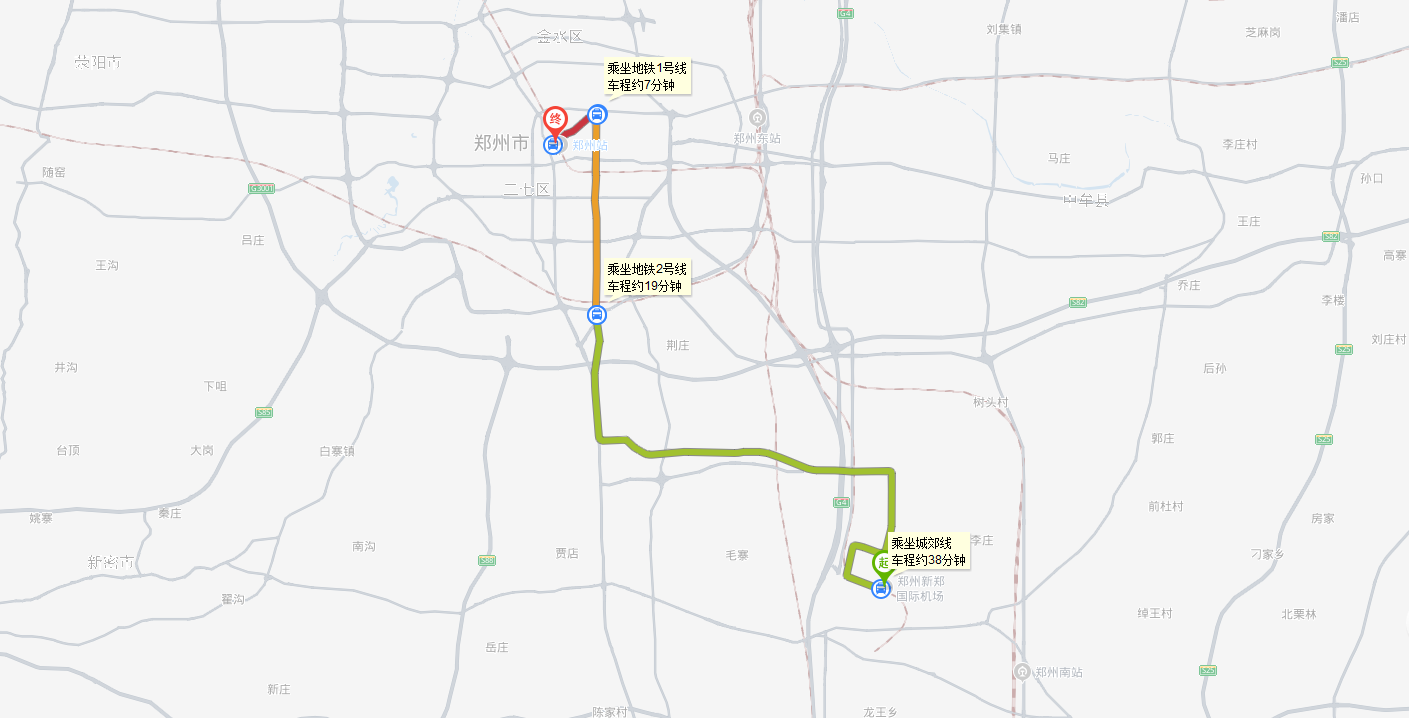
\includegraphics[width=0.8\textwidth]{Map_1.png}
	\caption{地图信息}
\end{figure}
根据地图查询结果得知:平均到市中心距离为:$50.7\mathrm{km}$,其中到高速路口距离为$l_{\mathrm{urban}}=35.7\mathrm{km}$,高速路口到市中心距离为$l_{\mathrm{city}}=15\mathrm{km}$\par
其中,由于满足式子:
\begin{equation}
	l_{\mathrm{city}}=v_{\mathrm{city}}\cdot t_{\mathrm{city}}
\end{equation}
所以有$ t_{\mathrm{city}} = \frac{l_{\mathrm{city}}}{v_{\mathrm{city}}}=30\mathrm{min} $

也即最终得到如下信息表格:\par
\begin{table}[!htbp]
	\caption[标签名]{得到的结果(部分)}
	\begin{tabular}{c|c|c|c|c|c|c|c|c}
		\toprule[1.5pt]
		$m_{\mathrm{start}}$ & $m_{\mathrm{oil}}$       & $l_{\mathrm{init}}$ & $v_{\mathrm{sub}}$            & $m_{\mathrm{night}}$ & $m_{\mathrm{aver}}$ & $l_{\mathrm{urban}}$ & $k$                    & $v_{\mathrm{city}}$  \\
		\midrule[1pt]
		8元                  & $0.4746$元$\mathrm{/km}$ & $2\mathrm{km}$      & $ \frac{5}{3}\mathrm{km/min}$ & $2$元                & $\frac{5}{6}$元     & $50.7\mathrm{km}$    & $ 1.5$元$\mathrm{/km}$ & $0.5\mathrm{km/min}$ \\
		\bottomrule[1.5pt]
		$t_{\mathrm{city}}$  & $v_{\mathrm{city}}$      &                     &                               &                      &                     &                      &                        &                      \\
		\midrule[1pt]
		$30\mathrm{min}$     & $0.5\mathrm{km/min} $    &                     &                               &                      &                     &                      &                        &                      \\
		\bottomrule[1.5pt]
	\end{tabular}
\end{table}
代入式子:
$$
	t_0=  \frac{fee(l_{\mathrm{urban}}+v_{\mathrm{city}} \cdot t_{\mathrm{city}})-m_{\mathrm{oil}}\cdot v_{\mathrm{city}} \cdot t_{\mathrm{city}}}{m_{\mathrm{aver}}} -t_{\mathrm{city}}
$$\par
当中,得到
$$
	t_0=  \frac{6}{5}\cdot(fee(50.7+0.5 \cdot 30)-0.4746\cdot 0.5 \cdot 30) -30= \frac{6}{5}\cdot fee(65.7)-38.5428
$$\par
则当为白天时,$t_0$为$t_0=85.7172\mathrm{min}$,当为夜班凌晨时,$t_0$为$t_0=88.1172\mathrm{min}$\par
由于加收夜补时间为22:00(含22:00)至次日5:00(含5:00),于是可以利用matlab绘制出图像,蓝色部分时间为司机应当继续排队等待接客,红色部分代表司机不应该继续排队,应当直接回到郑州市中心。\par
\begin{figure}[!h]
	\centering
	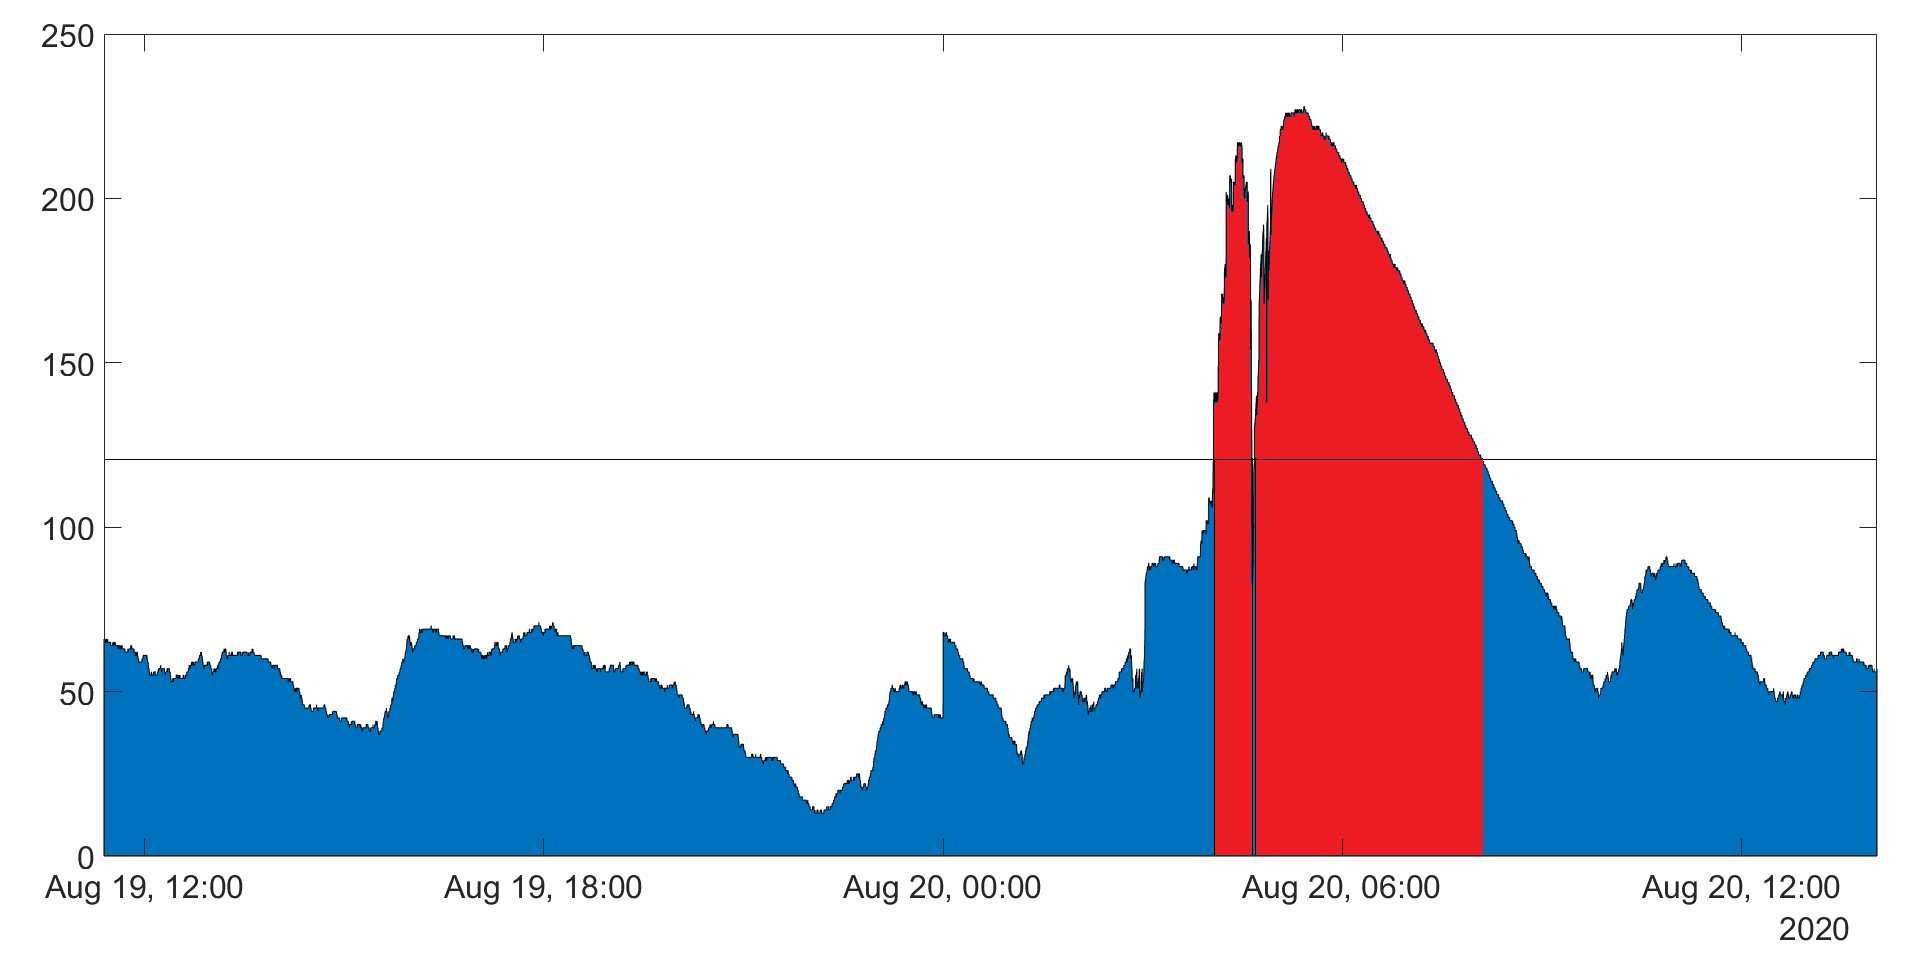
\includegraphics[width=1\textwidth]{Figure_6.png}
	\caption{}
\end{figure}
上面这幅图代表司机理应当做出的真正选择,但由于司机指能够根据他所见到的情景推算出大致的$t_{\mathrm{wait}}$,所以实际情况与应当选择的上一幅图是具有一定出入的,利用1问当中列举出的司机应当如何利用所得到的信息大致计算出还需要排多久。\par
收集到飞机航班信息之后,能够得到下图:\par \newpage
\begin{figure}[!h]
	\centering
	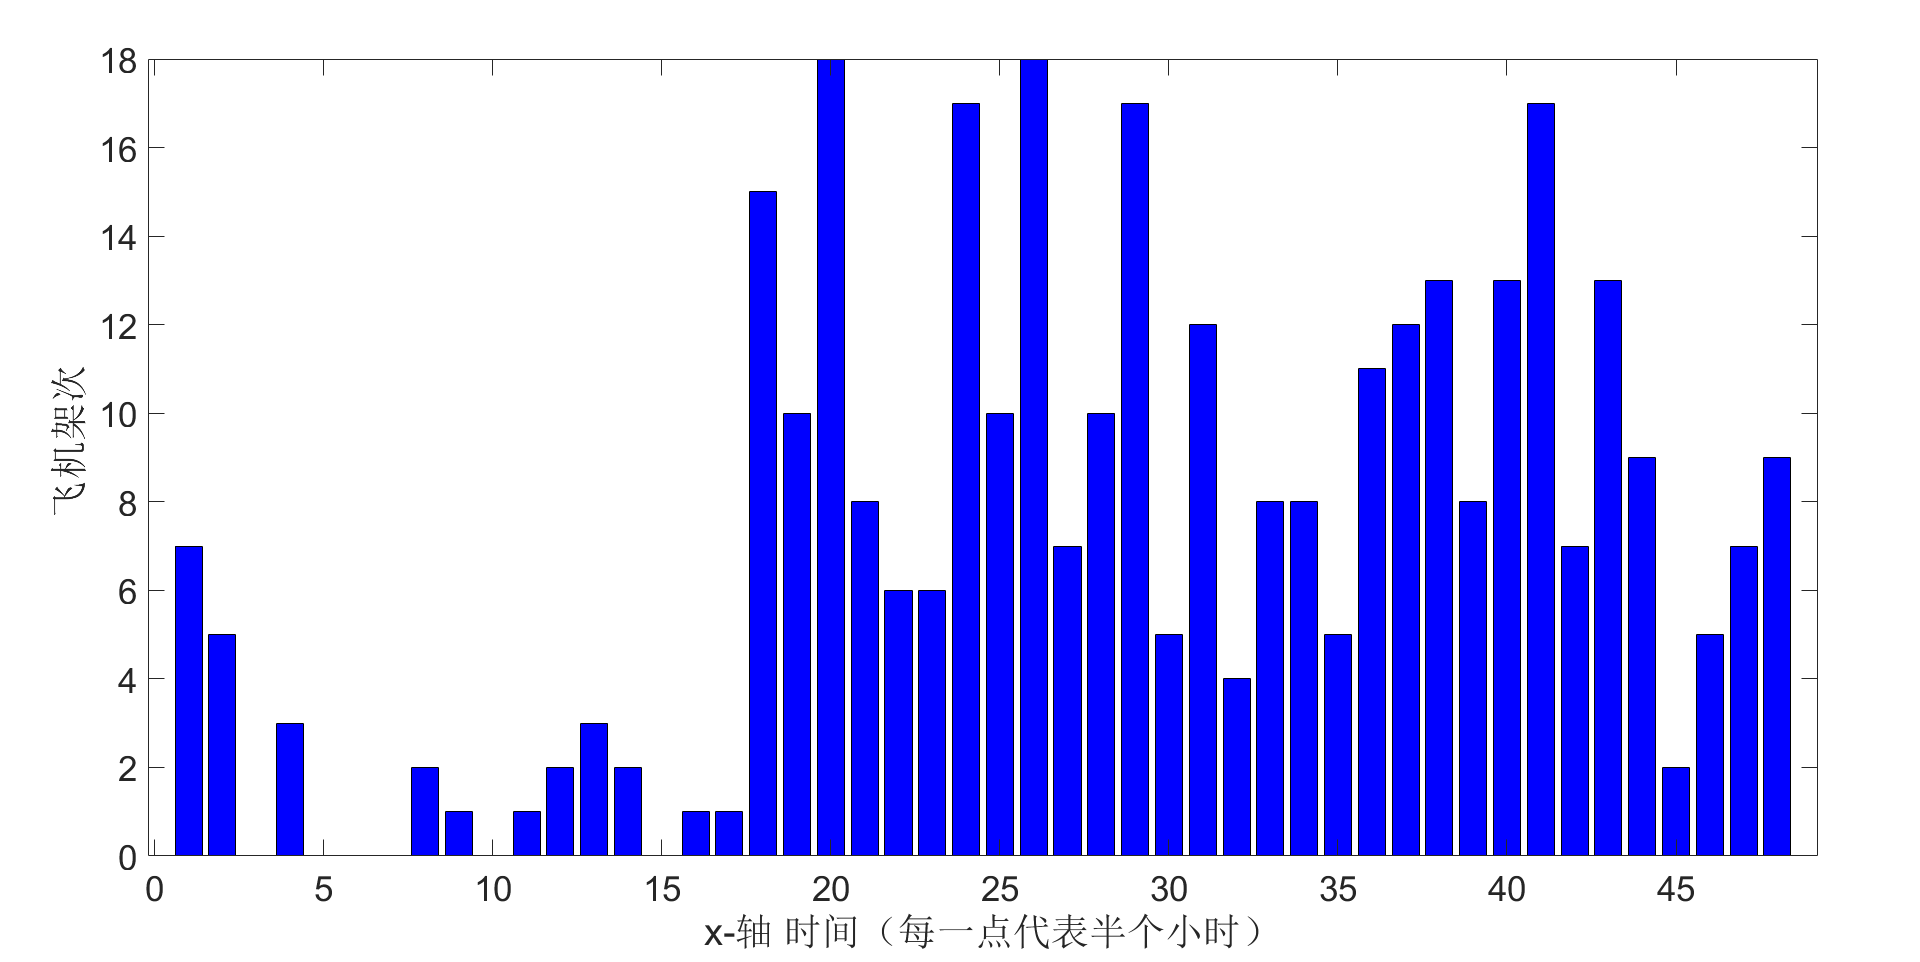
\includegraphics[width=1\textwidth]{Figure_8.png}
	\caption{}
\end{figure}
利用$v_{\mathrm{pin}}=\frac{n_{\mathrm{fly}}\cdot 300 \cdot \alpha}{30}$以及当不堆积或人堆积时有$t_{\mathrm{wait}}=\frac{n}{v_{\mathrm{out}}}$亦或者是人不堆积而车堆积时有$t_{\mathrm{wait}}=\frac{n}{v_{\mathrm{pin}}}$,我们能够得到司机在那个时刻根据具体情况所判断出来的$t_{\mathrm{wait}}$的值。\par

利用司机能够得知的内容与郑州市数据中心所产生的内容,也即下幅图片:\par
\begin{figure}[!h]
	\centering
	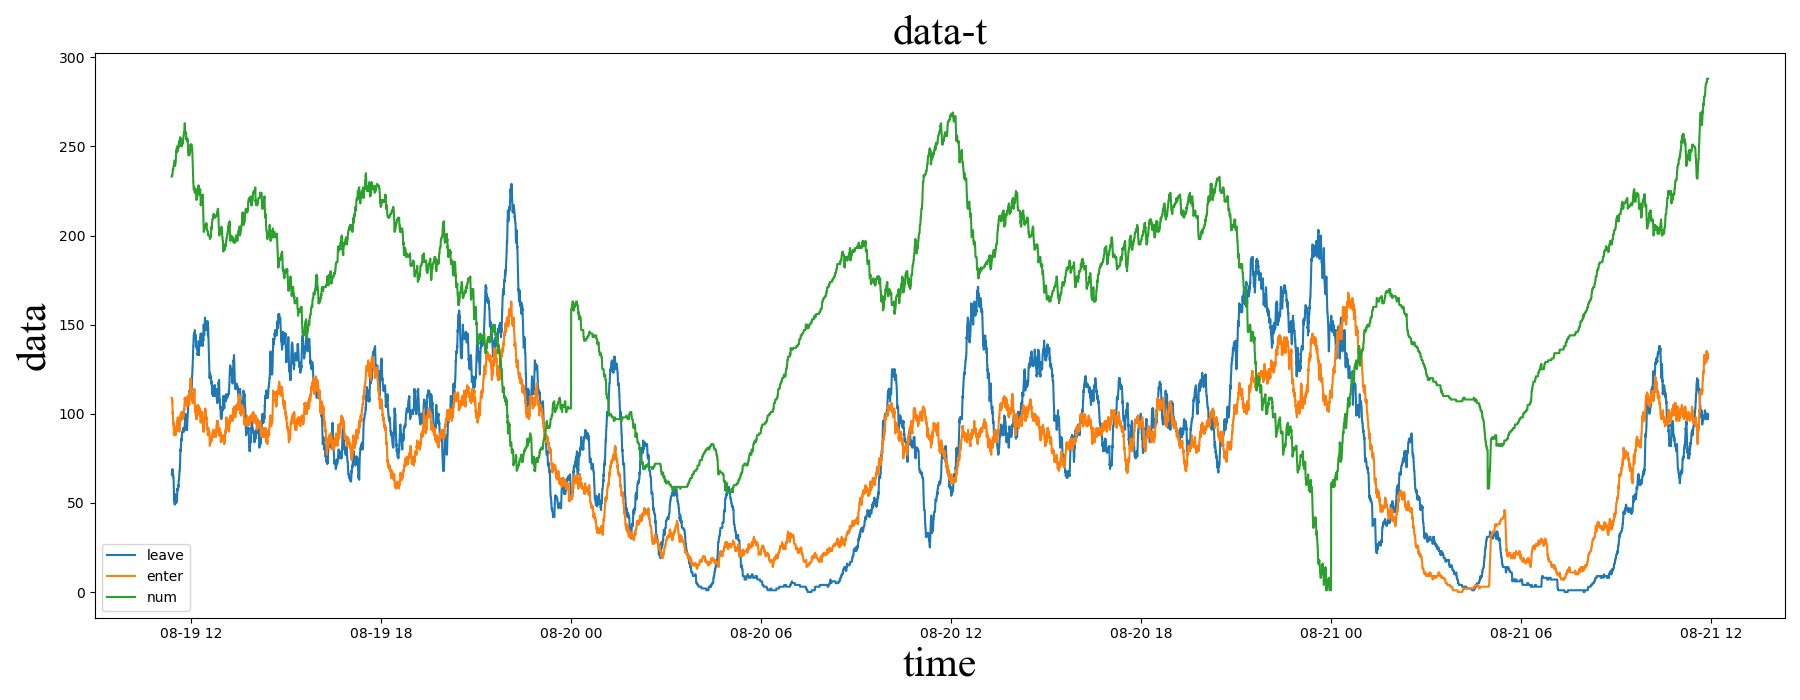
\includegraphics[width=1\textwidth]{datat.png}
	\caption{}
\end{figure}

结合matlab程序,得到司机所观测到的等待时间$t_{\mathrm{wait}}$,
其中,令$\alpha\sim\frac{1}{10}$,得出\par
\begin{figure}[!h]
	\centering
	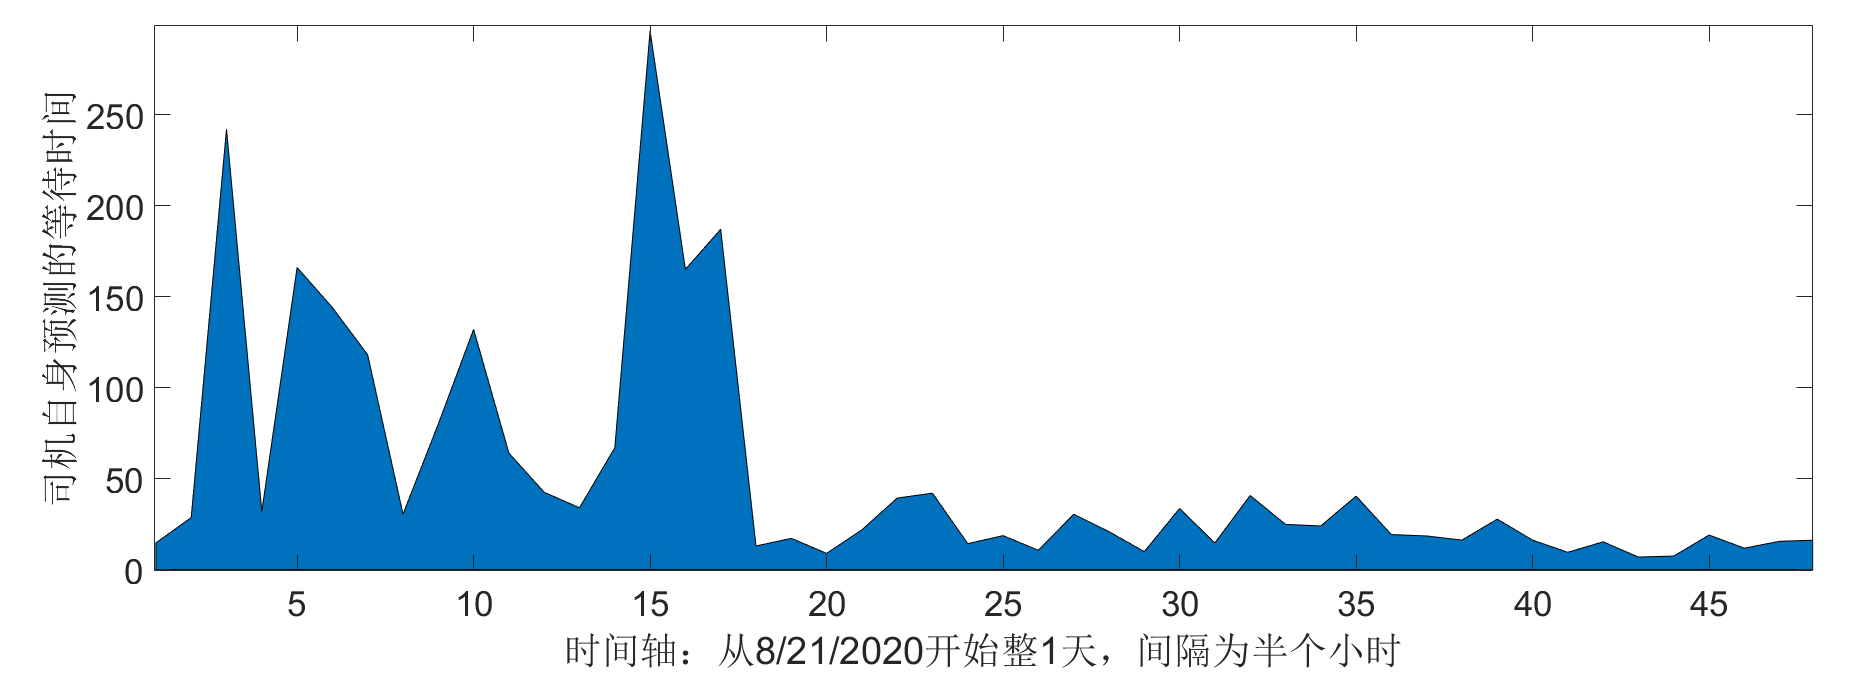
\includegraphics[width=1\textwidth]{Figure_9.png}
	\caption{}
\end{figure}
\newpage
依旧按照上图蓝色部分时间为司机应当继续排队等待接客,红色部分代表司机不应该继
续排队,应当直接回到郑州市中心的表示方法,利用 matlab绘制出图像。\par
则司机自身的选择会变成:\par
\begin{figure}[!h]
	\centering
	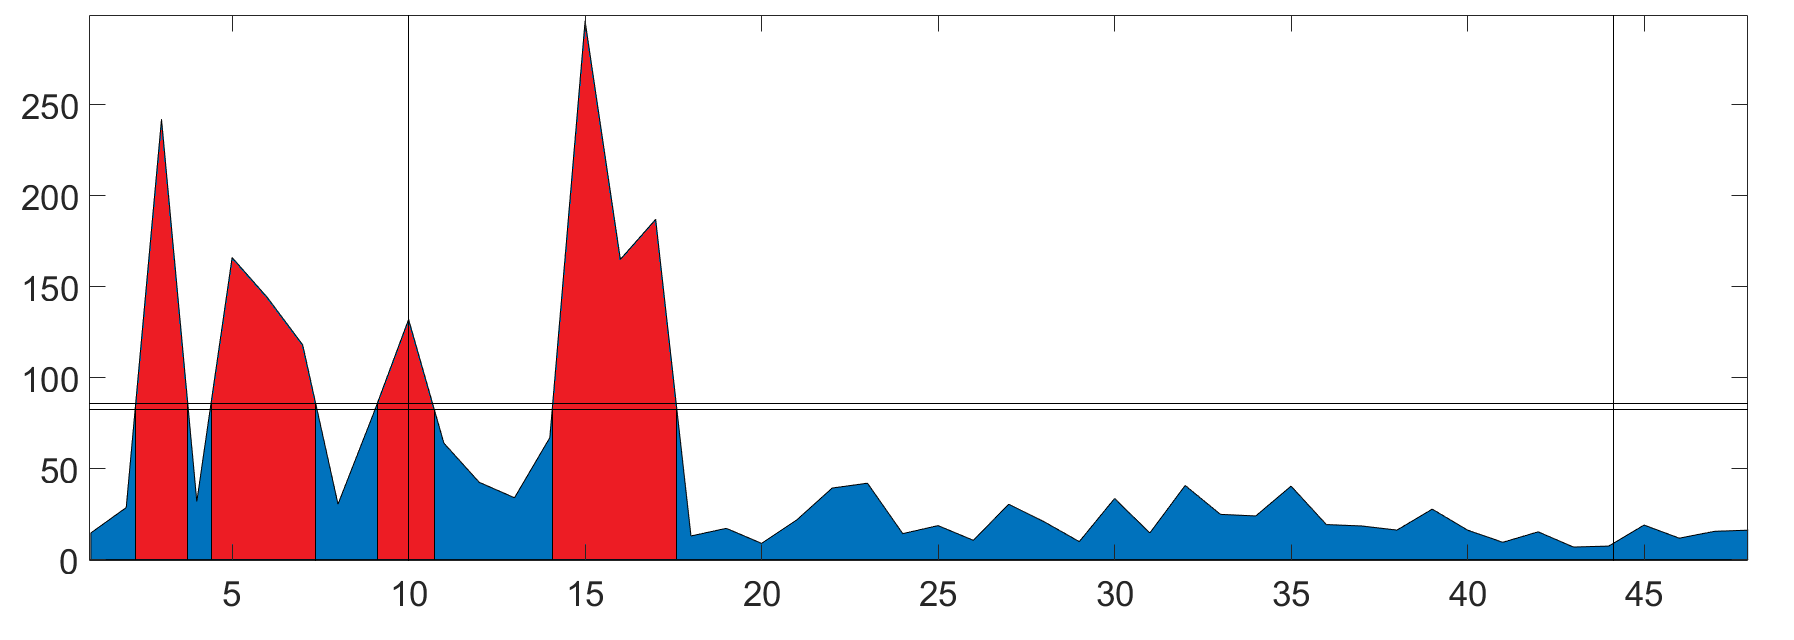
\includegraphics[width=1\textwidth]{Figure_10.png}
	\caption{}
\end{figure}


\newpage
\subsection{问题三的建模与求解}

\subsubsection{模型的建立}
第三问从机场管理部门角度出发,希望在有两条车道的前提下合理设置“上车点”,使得在保证车辆和乘客安全的条件下,使得总的乘车效率最高。\par
本文设置“上车点”的主要方案有以下几种:\par
1.控制“上车点”的数量,从而控制服务速度$v_{\mathrm{out}}$。\par
2.控制“上车点”的位置,从而控制蓄车池内出租车上限$N$。\par


\begin{figure}[!h]
	\centering
	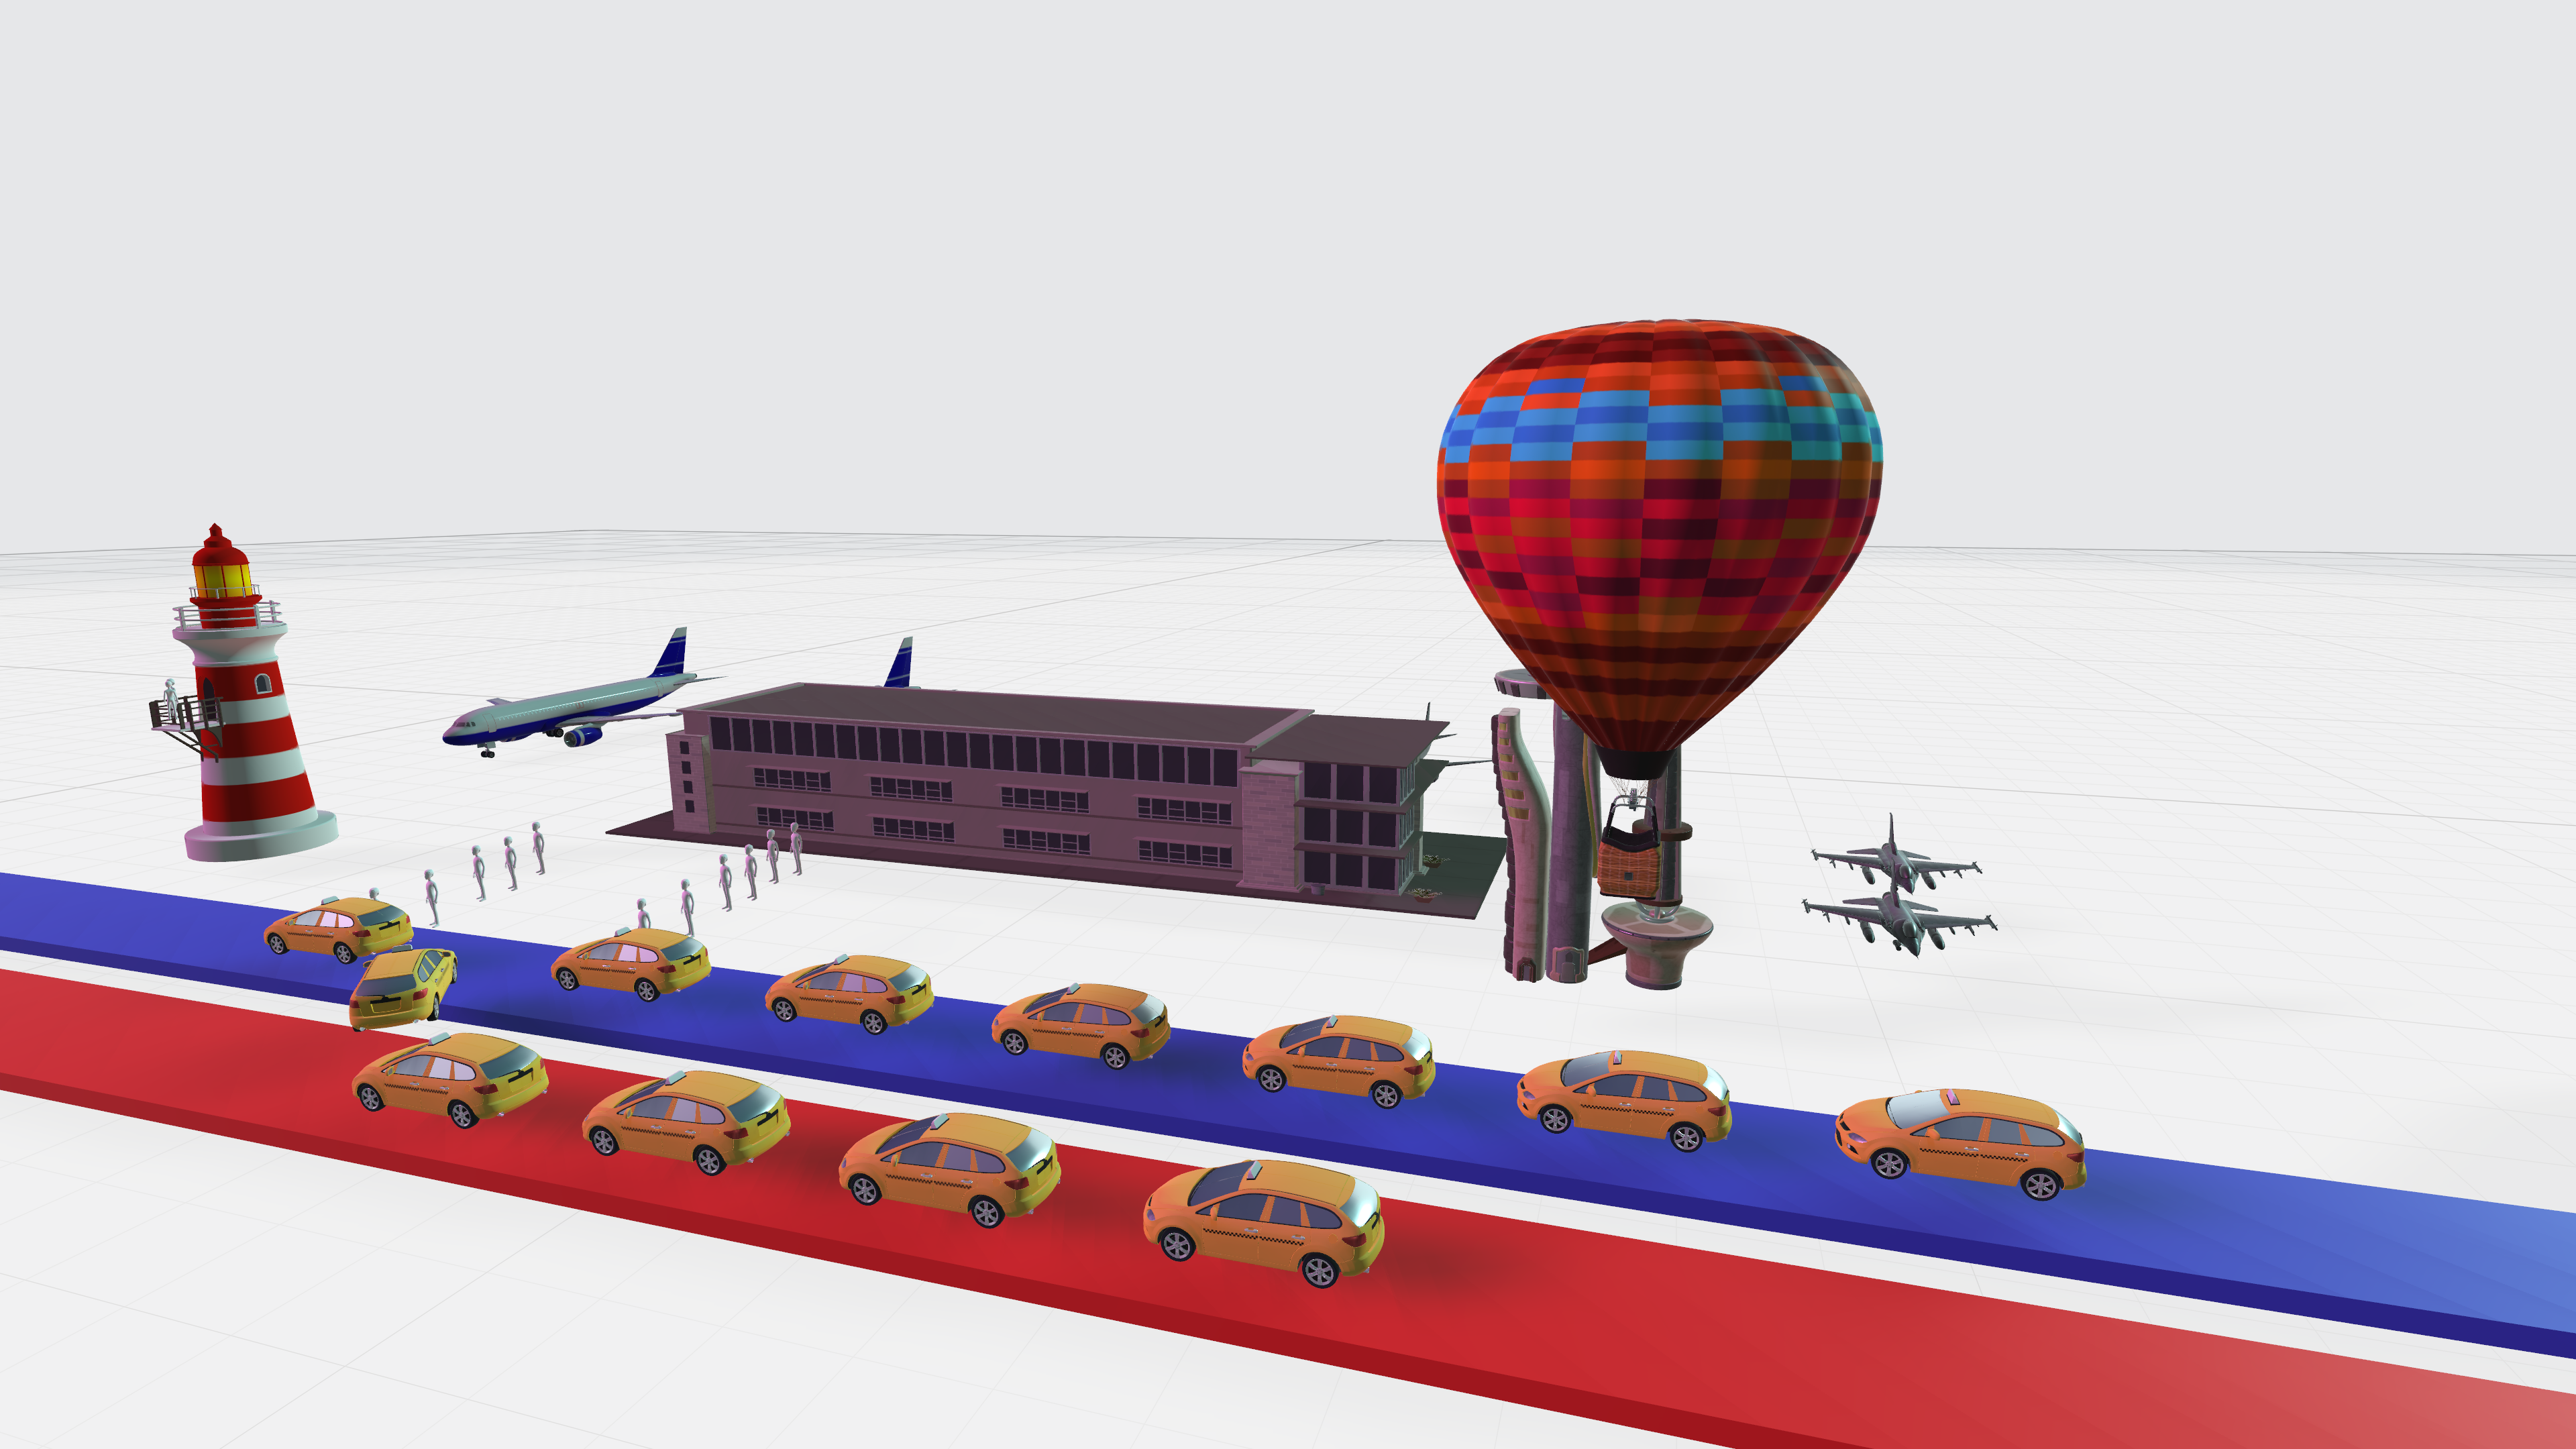
\includegraphics[width=1\textwidth]{case1.png}
	\caption{模拟送客示意图}
\end{figure}

\subsubsection{元胞自动机仿真模型}

为使得模型简单化,现只考虑蓄车池状态,并将蓄车池看成一个元胞。该元胞的主要参数为出租车数量$taxinum$。其转移过程如下图所示:
\begin{figure}[!h]
	\centering
	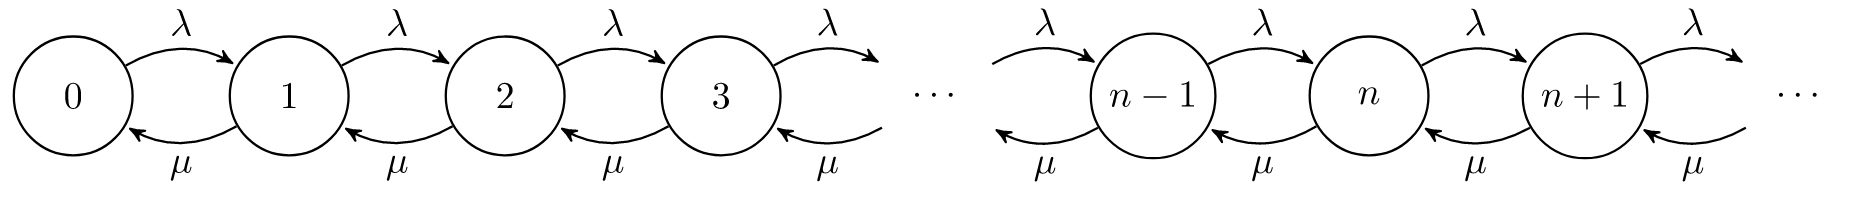
\includegraphics[width=1\textwidth]{元胞自动机模型.png}
	\caption{元胞转移过程}
\end{figure}

上图中$\lambda$为蓄车池增长概率,即单位时间元胞有$\lambda$概率增长1;图中$\mu$为服务概率,即单位时间元胞有$\mu$概率减小1。

如此,当“上车点”的数量增加,$\mu$值等比例增加。

为考察乘车效率,在此处定义流通系数:
\begin{equation}
	flu=\frac{servenum}{taxinum}
\end{equation}

上式中$servenum$为服务状态出租车数量。当总出租车数量增大时,流通系数减小;当服务数量增大时,在总出租车数量保持不变的情形下,流通系数增大。

假定初始态$\lambda=0.1$,$\mu=0.1$,$N=20$,用$python$程序模拟元胞变化过程,结果如下图所示:
\begin{figure}[!h]
	\centering
	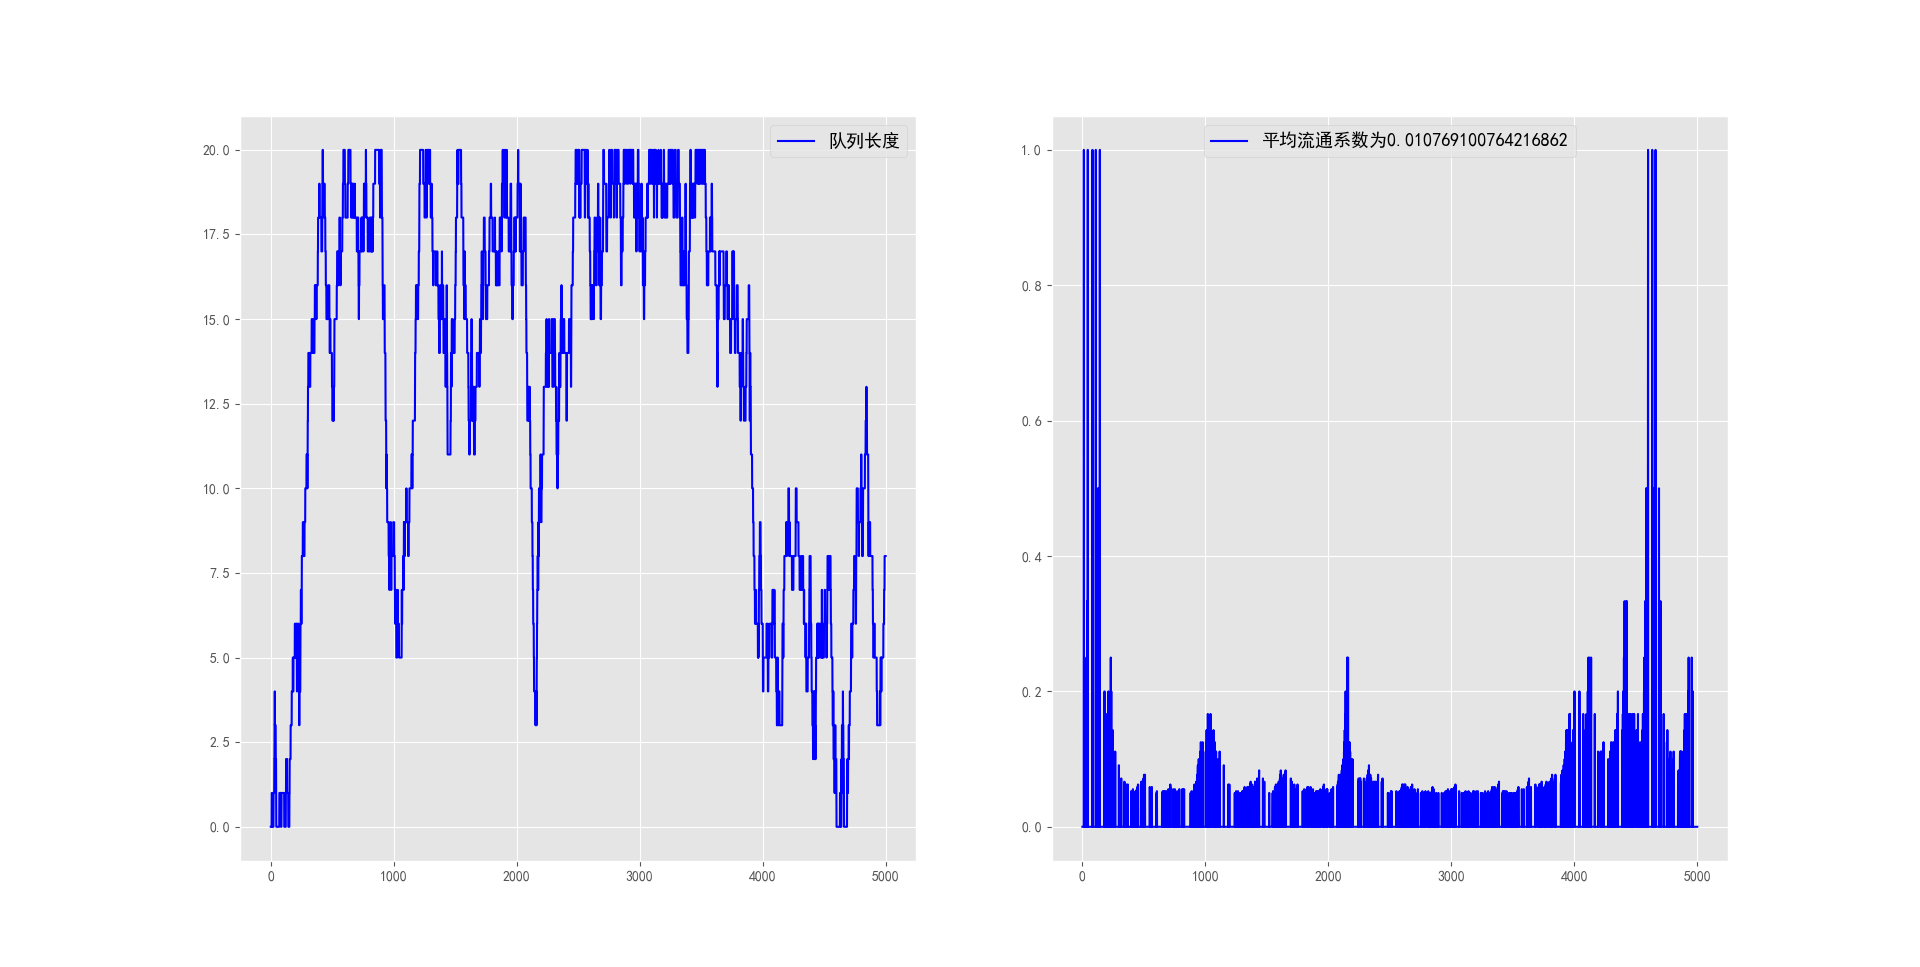
\includegraphics[width=1\textwidth]{YBresult1.png}
	\caption{元胞仿真结果1}
\end{figure}
\newpage

现考察改变“上车点”数量时,流通系数的变化如下表所示:
\begin{center}
	\begin{tabular}{cccc}
		\hline
		上车点数量 & 蓄车池上限 & $\mu$ & 平均流通系数 \\
		\hline
		1          & 20         & 0.1   & 0.0108       \\
		2          & 20         & 0.2   & 0.0724       \\
		3          & 20         & 0.3   & 0.0780       \\
		4          & 20         & 0.4   & 0.0856       \\
		5          & 20         & 0.5   & 0.0882       \\
		6          & 20         & 0.6   & 0.0926       \\
		\hline
	\end{tabular}
\end{center}

可发现,当固定蓄车池上限时,流通系数随上车点数量增加而增加,因而应在保证安全的情形下尽可能多安排上车点。

下面分析“上车点”位置即蓄车池上限对平均流通系数的影响,默认$\lambda=0.3$,$\mu=0.3$。
\begin{center}
	\begin{tabular}{cccc}
		\hline
		上车点数量 & 蓄车池上限 & $\mu$ & 平均流通系数 \\
		\hline
		3          & 20         & 0.3   & 0.0638       \\
		3          & 30         & 0.3   & 0.0652       \\
		3          & 40         & 0.3   & 0.0509       \\
		3          & 50         & 0.3   & 0.0318       \\
		3          & 60         & 0.3   & 0.0176       \\
		\hline
	\end{tabular}
\end{center}

会发现,确定上车点数量,当蓄车池上限增加时,总出租车数量可能性均值随之增加,因而流通系数下降。与实际情况相符。

根据以上分析,可以得到结论:应在保证安全的情形下提高上车点位置;降低蓄车池上限。

\subsubsection{模型的求解}



\newpage
\subsection{问题四的建模与求解}
\subsubsection{模型的建立}


\subsubsection{模型的求解}

\newpage
%参考文献
\begin{thebibliography}{9} % 宽度9
	\bibitem{bib:one} 参考文献
\end{thebibliography}

\newpage
%附录
\begin{appendices}

	\section{爬取郑州机场出租车管理站代码--C-sharp 源代码}
	\begin{lstlisting}[language=java]
using System;
using System.IO;
using System.Net;
using System.Text.RegularExpressions;
using System.Threading;

namespace c_2019
{
    internal class ResourcePool
    {
        public static string HttpGet(string Url, string contentType)
        {
            try
            {
                string retString = string.Empty;

                HttpWebRequest request = (HttpWebRequest)WebRequest.Create(Url);
                request.Method = "GET";
                request.ContentType = contentType;

                HttpWebResponse response = (HttpWebResponse)request.GetResponse();
                Stream myResponseStream = response.GetResponseStream();
                StreamReader streamReader = new StreamReader(myResponseStream);
                retString = streamReader.ReadToEnd();
                streamReader.Close();
                myResponseStream.Close();
                return retString;
            }
            catch (Exception ex)
            {
                return ex.Message;
            }
        }
    }

    class Program
    {
        static void Main(string[] args)
        {
            string head = "time,numbers,enter,leave";
            Console.WriteLine(head);
            using (StreamWriter file = new StreamWriter(@"val.csv", true))
            {
                file.Write(head);
            }
            for (; ; )
            {
                string ans = NetworkAirport.getContent();
                Console.WriteLine(ans);
                using (StreamWriter file = new StreamWriter(@"val.csv", true))
                {
                    file.WriteLine(ans);
                }
                Thread.Sleep(5000);
            }
        }
    }

    class NetworkAirport
    {
        public static string getContent()
        {
            try
            {
                string ans = "";
                string head = "http://www.whalebj.com";
                string content = ResourcePool.HttpGet(head + "/xzjc/default.aspx", "");

                string pattern = "截止目前为止([0-9]*-[0-9]*-[0-9]* [0-9]*:[0-9]*:[0-9]*)";
                MatchCollection mc = Regex.Matches(content, pattern);
                string time = mc[0].Value.Substring(7, 19);
                ans += time + ",";

                pattern = "场内待运车辆数为:[0-9]*";
                mc = Regex.Matches(content, pattern);
                string vehiclesNumColl = mc[0].Value.Substring(9);
                ans += vehiclesNumColl + ",";

                pattern = "前半小时进场车辆数为:[0-9]*";
                mc = Regex.Matches(content, pattern);
                vehiclesNumColl = mc[0].Value.Substring(11);
                ans += vehiclesNumColl + ",";

                pattern = "前半小时离场车辆数为:[0-9]*";
                mc = Regex.Matches(content, pattern);
                vehiclesNumColl = mc[0].Value.Substring(11);
                ans += vehiclesNumColl;

                return ans;
            }
            catch (Exception e)
            {
                return "";
            }
        }
    }
}

\end{lstlisting}

	\section{爬取郑州机场航班信息代码--JavaScript 源代码}
	\begin{lstlisting}[language=java]
console.log('"载体","飞行","起源","状态","到来"');

function getarrivals(){
    for (let i = 1; i < 9; i++) {
        setTimeout(() => {
            var timeperiod = document.getElementsByClassName("timeperiod");
            var timeperiodNode = timeperiod[0].childNodes
            var shouldClick = timeperiodNode[i * 2];
            shouldClick.click();
            setTimeout(() => {
                var arrivals = document.getElementById("arrivals");
                var nodeColl = arrivals.childNodes;
                for (let j = 0; j < nodeColl.length; j++) {
                    var subTempText = "";
                    var airData = nodeColl[j].childNodes;
                    for (let k = 0; k < airData.length - 1; k++) {
                        var text = airData[k].childNodes[0].textContent;
                        subTempText += '"' + text + '"' + ',';
                    }
                    subTempText += '"' + airData[airData.length - 1].childNodes[0].textContent + '"';
                    console.log(subTempText);
                }
            }, 5000);
        }, i * 6000);
    }    
}

function getdepartures(){
    for (let i = 1; i < 9; i++) {
        setTimeout(() => {
            var timeperiod = document.getElementsByClassName("timeperiod");
            var timeperiodNode = timeperiod[0].childNodes
            var shouldClick = timeperiodNode[i * 2];
            shouldClick.click();
            setTimeout(() => {
                var departures = document.getElementById("departures");
                var nodeColl = departures.childNodes;
                for (let j = 0; j < nodeColl.length; j++) {
                    var subTempText = "";
                    var airData = nodeColl[j].childNodes;
                    for (let k = 0; k < airData.length - 1; k++) {
                        var text = airData[k].childNodes[0].textContent;
                        subTempText += '"' + text + '"' + ',';
                    }
                    subTempText += '"' + airData[airData.length - 1].childNodes[0].textContent + '"';
                    console.log(subTempText);
                }
            }, 5000);
        }, i * 6000);
    }    
}

\end{lstlisting}

	\section{第二小问解题方法及绘图--Matlab 源代码}
	\begin{lstlisting}[language=Matlab]
time = val.time;
numbers = val.numbers;
enter = val.enter;
leave = val.leave;

e = enter / 30;
l = leave / 30;

t_wait = 1:18000;

%initializing the t_wait
interval = 12

for i=1:18000
    t_wait(1:i)=0;
end


%the main code
for i=1:18000
    temp = 0;
    for j=1:18000
        if  temp >= numbers(i,1)
            t_wait(i) = j;
            break
        else 
            temp = temp + l(j * interval + i,1);
        end
    end
end


time_temp = time(1:18000).';
area(time_temp,t_wait,'DisplayName','t_wait')
xlim([time_temp(1,1)  time_temp(1,18000)])

area(time,l,'DisplayName','l')
xlim([time_temp(1,1)  time(20282)])
area(time,numbers,'DisplayName','numbers')
xlim([time_temp(1,1)  time(20282)])


time_arr =  arrival.time;
status = arrival.status;

t = 1/48

data = 1:48;

for i=1:48
    data(1,i) = 0;
end

for i=1:48
    temp = 0;
    for j=1:368
        if time_arr(j) > (t*(i-1))
            if time_arr(j) < (t*i)
                temp = temp + 1;               
            end
        end
    end
    data(1,i) = temp
end

plot(xx,data)
bar(xx,data,'DisplayName','data')


START = 8531

GAP = 360

t_wait_t = 1:48;

for i=1:48
    t_wait_t(i) = 0; 
end

for i=1:48
    num = data(1,i);
    if num == 0
        num = 0.5;
    end
    t_wait_t(i) = numbers(START+(i-1)*GAP) / num
end


>> xx = 1:48;
>> histogram(t_wait_t,xx)
>> area(xx,t_wait_t,'DisplayName','t_wait_t')
>> area(xx,t_wait_t,'DisplayName','t_wait_t')
>> xlim([0.5 48])
>> xlim([1 48])
\end{lstlisting}





\end{appendices}

\end{document}